\documentclass[9pt,twoside,lineno]{pnas-new}
% Use the lineno option to display guide line numbers if required.

\templatetype{pnasresearcharticle}
\usepackage{longtable}
\usepackage{array,ragged2e} % for nicer justification of table entries with "P"
\newcolumntype{P}[1]{>{\RaggedRight\arraybackslash}p{#1}}
\usepackage{caption} % for subfigures
\usepackage{subcaption}
\usepackage{lscape} % for turning one page to landscape

\let\thefigureWithoutS\thefigure %% <- store old definition
\renewcommand\thefigure{S\thefigureWithoutS}

\usepackage[backend=bibtex,style=nature]{biblatex}
\bibliography{references}

\newcommand\focalcountry{CHE}
\newcommand\mindate{01. Jan. 2020}
\newcommand\maxdate{01. Dec. 2020}
\newcommand\maxmissing{2903}
\newcommand\minlength{27000}
\newcommand\maxsamplingfraction{0.05}
\newcommand\subsamplebycanton{TRUE}
\newcommand\travelcontextscalefactor{0}
\newcommand\similaritycontextscalefactor{2}
\newcommand\traveldataweights{1,1,1}
\newcommand\whichtrees{\.*}
\newcommand\pickchainsunderothercriteria{TRUE}
\newcommand\ntrees{-1}
\newcommand\smoothconfcases{FALSE}
\newcommand\outgroupgisaidepiisls{EPI\_ISL\_406798}
\newcommand\uniquecontextonly{FALSE}
\newcommand\maskfromstart{100}
\newcommand\maskfromend{50}

\newcommand\nchainsmin{746}
\newcommand\nchainsmax{2995}
\newcommand\minlargestchainsper{23}
\newcommand\maxlargestchainsper{14}
\newcommand\nspanningchainsmin{}
\newcommand\nspanningchainsmax{}

\newcommand\nfocalsamples{5520}
\newcommand\nsimcontext{11009}
\newcommand\ntravelcontext{0}
\newcommand\meanweeklysamplingpercent{NaN}
\newcommand\minweeklysamplingpercent{NaN}
\newcommand\maxweeklysamplingpercent{NaN}
\newcommand\overallsamplingpercent{1.4}

\newcommand\summer_max_dampling_percent_median_CHE_no_sampUB{37}
\newcommand\summer_min_dampling_percent_median_CHE_no_sampUB{65}

\newcommand\medpersistenceatlockdownmin{27.5}
\newcommand\medpersistenceatlockdownmax{0}
\newcommand\qonepersistenceatlockdownmin{5.75}
\newcommand\qonepersistenceatlockdownmax{0}
\newcommand\qthreepersistenceatlockdownmin{58.5}
\newcommand\qthreepersistenceatlockdownmax{1}
\newcommand\medpersistenceatpeakmin{174}
\newcommand\medpersistenceatpeakmax{167}
\newcommand\qonepersistenceatpeakmin{163}
\newcommand\qonepersistenceatpeakmax{111}
\newcommand\qthreepersistenceatpeakmin{192}
\newcommand\qthreepersistenceatpeakmax{169.5}

\newcommand\casescoeffmax{0.048}
\newcommand\casescoeffmin{0.0074}
\newcommand\casesdelaymax{2}
\newcommand\casesdelaymin{5}
\newcommand\introsavertedmax{4038}
\newcommand\introsavertedmin{593}
\newcommand\introsavertedaspermax{84}
\newcommand\introsavertedaspermin{83}


\usepackage{xfp} % to do multiplication with \inteval
\newcommand{\maxsamplingpercent}{\maxsamplingfraction*100}

\title{Supporting information}
\author{}
% \correspondingauthor{Corresponding Author name.\\E-mail: author.two@email.com}

\begin{document}

\maketitle 

\tableofcontents

\newpage

\section{Materials and methods}
\subsection{Genome sequencing and quality filtering}
Most of the Swiss SARS-CoV-2 genomes analyzed until 31. Dec 2020 were generated by the Swiss SARS-CoV-2 Sequencing Consortium \cite{s3c-webpage}. Here, we briefly describe the swab-to-sequence process for these samples. RNA extracts from qPRC-positive patient naso- or oral-pharangeal swabs were provided by Viollier AG, a Swiss medical diagnostics company. RNA extraction was done with either the Abbott m2000sp or Seegene STARMag 96x4 Universal Cartridge RNA extraction kit. Extracts were then  transferred to the Genomics Facility Basel or the Functional Genomics Center Zurich for whole-genome sequencing. Both centers used the ARCTIC v3 primer scheme \cite{Quick2017, ARCTICNetwork} to generate tiled, approximately 400bp-long amplicons. Library preparation was done with the New England Biolabs (NEB) library preparation kit. Libraries were sequenced on Illumina MiSeq or NovaSeq machines, resulting in 2 x 251 base reads. Bioinformatics was done using V-pipe \cite{v-pipe-bioinformatics}, including read trimming and filtering with PRINSEQ \cite{Schmieder2011}, alignment to GenBank accession MN908947 \cite{Wu2020} with bwa \cite{Li2009}, and consensus base calling. For consensus base calling, positions with $<$5x coverage are masked with ``N'', positions with $>$5\% and $>$2 reads supporting a minor base are called with IUPAC ambiguity codes, and positions with $>$50\% reads supporting a deletion are called with ``-''. We rejected samples with $<$20,000 non-N bases. The consensus sequences we generated have been made publicly available on both GISAID (submitting lab: Department of Biosystems Science and Engineering, ETH Zürich) and European Nucleotide Archive (ENA) (study: PRJEB38472).

We supplemented our Swiss data with other Swiss sequences and foreign sequences available via GISAID (accessed 31. May 2021). From the full set of sequences available on GISAID, we removed from consideration non-human samples, samples $<$ 27000 bases long, and samples flagged by the Nextclade tool \cite{Aksamentov} for one of the following reasons: suspiciously clustered SNPs (QC SNP clusters status metric not ``good''; $>=$ 6 mutations in 100 bases), too many private mutations (QC private mutations status metric not ``good''; $>=$ 10 mutations from the nearest tree node), or overall bad quality (Nextclade QC overall status ``bad''). We aligned the sequences to the reference genome MN908947.3 using MAFFT \cite{katoh_mafft:_2002}. Finally, we followed the Nextstrain pipeline's recommendation to mask the first 100 and last 50 sites of the alignment \cite{Nextstraina} since the start and end of SARS-CoV-2 sequences are prone to sequencing error \cite{DeMaio2020}.

\subsection{Sampling procedure}

From the quality-filtered alignment of GISAID sequences, we selected a focal set of sequences from Switzerland and a context set of sequences from abroad. 

% describe representativeness of Swiss dataset here too?
For the focal sequences from Switzerland, we aimed to select a spatially and temporally representative sample. Therefore, we down-sampled available sequences to \fpeval{\maxsamplingpercent}\% of confirmed case counts in each Swiss Canton each week between \mindate\ and \maxdate. Where there were not enough sequences available from a Canton in a week, we took all available sequences. To reduce the size of the alignments for phylogenetic analysis, we divided the focal Swiss set into Pango lineages \cite{Rambaut}, similar to \cite{DuPlessis2021}. Lineages composed of $>$ 50\% Swiss sequences were aggregated into their parent lineage(s) until $<=$ 50\% were Swiss. This aims to ensure that each analyzed lineage originated outside of Switzerland.

% describe nextstrain priority protocol for sim dataset
For the contextual sequences from abroad, we aimed to select the most genetically similar sequences to focal Swiss sequences. This set should help distinguish between SARS-CoV-2 variants unique to Switzerland (likely within-Switzerland transmission) and variants also circulating abroad (possibly recent introductions). To select this set, we applied the Nextstrain priority script \cite{Nextstrainteam} to rank sequences from abroad by their genetic similarity to Swiss sequences in each lineage alignment. Then, we selected \similaritycontextscalefactor\ times as many  context sequences as focal Swiss sequences for each analyzed lineage. 

% summarize the sample set
In the supporting information, we show sensitivity analyses for these choices. We tested different numbers of focal Swiss sequences and different ratios of contextual to focal sequences, with the conclusion that the most variation is still due to how we define an introduction (see ``Identifying introductions'', below). The final dataset used for analysis includes \nfocalsamples\ focal sequences from Switzerland and \nsimcontext\ genetically similar contextual sequences from abroad.

\subsection{Timetree generation}
We estimated the maximum likelihood phylogeny for each lineage alignment using IQ-TREE \cite{Nguyen2014} under an HKY substitution model \cite{Hasegawa1985} with empirical base frequencies and 4 gamma rate categories. We then rooted each phylogeny with \outgroupgisaidepiisls\ as an outgroup and estimated branch lengths in time units using least-squares dating (LSD) \cite{To2016} with a strict molecular clock and a minimum mutation rate of 8x10-4 substitutions per site per year. We additionally assumed the root date to be between 15. Nov. and 24. Dec. 2019 (roughly in line with estimates provided by Nextstrain \cite{Nextstrainteam}) and set the minimum branch length to zero. Sequences that violated the strict clock assumption (z-score threshold > 3) were removed and near-zero branches ($<$1.7x10-5 substitutions per site per year) were collapsed into polytomies, reflecting the fact that the sequence data is not sufficient to resolve the ordering of these transmission events. Given the root date constraints, the mutation rate conformed to the lower bound of 8x10-4 with extremely narrow confidence intervals. Confidence intervals for node dates were generated in LSD by re- sampling branch lengths 100 times under a lognormal relaxed clock model with standard deviation 0.4.

\subsection{Identifying introductions}
We ``picked'' putative Swiss transmission chains (collections of two or more genomic sequences resulting from within-Switzerland transmissions) off of each Pango lineage tree according to the following criteria: at least 2 Swiss sequences are part of a clade in the tree and the subtree spanned by these Swiss sequences is monophyletic upon removing (a) up to 3 export events where (b) only one export event may occur along each internal branch. Exports are defined to be clades containing non-Swiss sequences. We chose a conservative value for criterion (b) while still allowing some export events and note that the number of inferred transmission chains is robust to different values for criterion (a) given criterion (b) (Fig. \ref{fig:sensitivity_figs}c). For a sensitivity analysis on the importance of the specific values of criteria (a) and (b) see the supporting text.

We refer to any Swiss sequence not falling into a Swiss transmission chain as a Swiss singleton. We assume each singleton and each transmission chain represent an independent introduction of SARS-CoV-2 into Switzerland; together these are called introductions.

Finally, we repeated this picking procedure twice for each lineage tree, interpreting polytomies in two different ways. Once, we split Swiss clades descending from polytomies into independent introductions unless the polytomy only had a single non-Swiss descendent (see criterion (b)). Alternatively, we aggregated all Swiss clades descending from polytomies into a single introduction. These procedures are conceptually similar to the ACCTRANS (accelerated transformations) and DELTRANS (delayed transformations) methods for assigning character transformations when multiple scenarios are equally parsimonious \cite{Miyakawa2004}. In summary, we identify introductions twice, generating estimates that represent two plausible extremes of  many introductions and few introductions.

\subsection{Quantifying the effect of border closures on introductions}
We wanted to understand if the Swiss border closure on 13 Mar. 2020 changed introduction dynamics. Our null model is that the number of weekly introductions before border closure, estimated from the genome data as described above, is a linear function of weekly SARS-CoV-2 cases in surrounding countries. Introductions are dated by the first detected case, whereas case counts (taken from the ECDC \cite{ECDC}) are dated by case reporting dates. We considered an average delay between these variables up to 18 days. We also considered two options for ``surrounding countries'', either all the non-Swiss European countries in the ECDC dataset or just Switzerland's neighboring countries Italy, France, Germany, and Austria. We fit these models separately to the weekly many and few introductions estimates before 13 Mar. 2020 and selected the best-fit models (lowest root mean squared error). For both estimates, the neighboring-countries-only incidence data better predicted introductions. The best-fit delay was \casesdelaymax days for the many introductions estimates compared to \casesdelaymin days for the few introductions estimates. Figure \ref{fig:introductions_and_persistence_v2} shows these best-fit models and projections if these dynamics had continued after 13. Mar.

\subsection{Quantifying the effect of lockdown conditions on persistence}
We also wanted to understand if the Swiss lockdown between 17 Mar. and 27 Apr. 2020 changed the persistence of introductions. Our null model is that introductions circulating on any given day persist equally long, regardless of the day. In other words, introductions die out (are no longer sampled) according to some delay distribution that is constant through time. For each date, we calculated the median and inter-quartile range of the time from that date to the last sample for all introductions persisting on that date. Singleton introductions trivially persist for 1 day. Figure \ref{fig:introductions_and_persistence_v2} shows how the persistence of the estimated introductions changes around the dates of the Swiss lockdown from 17. Mar to 27. Apr.

\subsection*{Phylodynamic analysis}

After identifying introductions, we performed phylodynamic inference on them using the BDSKY (birth-death skyline) method \cite{stadler2013birth} in BEAST2 \cite{Bouckaert2019}. To avoid model mis-specification due to the more transmissible alpha variant, we analyzed data only through 30 Nov.~2020.  The inference relies on two main models: a nucleotide substitution model describing an evolutionary process and a population dynamical model describing a transmission and sampling process. 

For the nucleotide substitution model, we assumed an HKY \cite{Hasegawa1985} model with 4 Gamma rate categories to account for site-to-site rate heterogeneity \cite{Yang1994}. We used the default priors for kappa and the scale factor of the Gamma distribution. We assumed a strict clock with rate $8\times 10^{-4}$ substitutions per site per year.

For the population dynamic model, we used BDSKY \cite{stadler2013birth}. In BDSKY, the identified introductions are the result of a birth-death with sampling process parameterized by an effective reproductive number, a becoming-uninfectious rate, and a sampling probability. As in \cite{Muller2020}, we inferred these population dynamical parameters jointly from the different introductions. More concretely, each introduction is assumed to result from an independent birth-death process having its own start time, but sharing all other parameters with the processes associated with the other introductions. 
Further, we used a uniform prior on the time of origin for each introduction, from 01. Jan until the end of the sampling period. This means our prior expectation is a uniform rate of introductions through time. We fixed the become-uninfectious rate to 36.5 per year, which corresponds to an average of 10 days to becoming uninfectious. We allowed the effective reproductive number to vary week-to-week. We applied an Ornstein-Uhlenbeck smoothing prior to the logarithm of this parameter, defined such that the stationary distribution of the process was $\text{LogNormal}(0.8, 0.5)$  and with an $\text{Exp}(1)$ hyperprior on the relaxation parameter of the process. This prior constrains both the absolute reproductive number and the relative sizes of the change between weeks. Finally, we allowed the sampling probability to vary when Swiss testing or genome sampling regimes changed significantly (Table S1). For our main analysis, we applied a $\text{LogUniform}(10^{-4}, 1)$ prior on the sampling probability. As a sensitivity analysis, we also tried a $\text{LogUniform}(10^{-4}, 0.05)$ prior since we upper-bounded our sampling to 5\% of confirmed cases each week. See the supporting text for more information.

Then, we added an additional ``contact tracing'' factor to the model. This factor is a multiplicative damping of the effective reproductive number applied to each introduction from 2 days after the first sample date until the introduction dies out. Since we hypothesized contact tracing was not functioning as well during periods of high case numbers, we estimated a separate value in each of three periods: before 15. Jun 2020 (Spring), 15 Jun.~to 30 Sept.~2020 (Summer), and 30. Sept to \maxdate\ (Fall). We used the same spike and slab prior for the damping factor in each period, with an inclusion probability of 0.5 and a uniform prior if included between 0 and 1. 

The XML files for the phylodynamic analysis are available on the project GitHub repository at TODO.

\section{Supporting text}

% \subsection*{Subhead}
% Type or paste text here. This should be additional explanatory text such as an extended technical description of results, full details of mathematical models, etc.   
\subsection{Sensitivity analyses for identifying introductions}
Here we describe different sensitivity analyses we performed for the definition of an introduction. 

\subsubsection{Number of focal Swiss sequences analyzed}
To assess whether the number of identified introductions saturates as we add more sequences, we did a sub-sampling analysis. We sub-sampled the Swiss genome sequences used in our main analysis from 5\% of confirmed cases down to 1\% of confirmed cases. For each new sub-sampling value, we calculated the number of introductions (singletons and transmission chains) that we would have identified given the sub-sampled sequence set. Figure \ref{fig:sensitivity_figs}a shows that as we add sequences, we do not reach saturation. Therefore, if we were to include even more sequences, we would almost certainly identify more introductions into Switzerland.

\subsubsection{Ratio of foreign context to focal Swiss sequences analyzed}
Next, we assessed how summary statistics about identified introductions and the runtime of our pipeline changed as we added more and more foreign context sequences. We kept the number of focal Swiss sequences constant at 5\% of confirmed cases each week and added foreign context sequences at a 1:1, 2:1, and 3:1 ratio to focal Swiss sequences. Figure \ref{fig:sensitivity_figs}b shows that as we add foreign context sequences, we identify more numerous, smaller introductions. However, the greatest differences come from the different assumptions about how to resolve polytomies (few vs. many introductions), not the ratio of foreign context to focal Swiss sequences. Therefore, we chose to present results using the 2:1 ratio to balance speed (smaller dataset = faster tree search convergence) and information content (larger dataset = more precise estimates of introduction dates).

\subsubsection{Criteria for identifying introductions}
After deciding on a ratio of foreign context to focal Swiss sequences, we assessed how summary statistics about identified introductions changed depending on the precise heuristic definition of an introduction. Given phylogenetic trees with polytomies, we picked transmission chains off of these trees as described in the main text methods. Here, we varied (a) the number of export events allowed in each transmission chain and (b) the maximum number of export events allowed to occur along each single internal branch. Figure \ref{fig:sensitivity_figs}c shows that increasing (a) yields fewer, larger transmission chains. Increasing (b) for each level of (a) has a much smaller effect. We note that again, the greatest differences come from the different assumptions about how to resolve polytomies. Therefore, we chose to present results using a transmission chain definition based on (a) maximum 3 exported lineages and (b) maximum one consecutive export on each internal branch. This allows for some exports from Swiss transmission chains but not arbitrarily many. 

\subsection{Sensitivity analyses for phylodynamic modelling}
Here we describe a sensitivity analyses and some example intermediate outputs from our phylodynamic analysis.

\subsubsection{Sampling proportion prior}
We wanted to check that our phylodynamic estimates of a transmission damping factor are robust to our prior on the sampling proportion. Therefore, we repeated our analyses using two different priors on the sampling proportion. The first prior was a uniform distribution between 0 and 1. This broad prior allows the sampling proportion to assume any plausible value. The second prior was a uniform distribution between 0 and an upper bound equal to the number of genome sequences analyzed in a week divided by the number of confirmed cases that week. This narrower prior assumes that there are at least as many cases each week as confirmed cases. Figure \ref{fig:ReSampProbResults}a shows that in Switzerland, the estimated sampling proportion in late Fall 2020 varies greatly depending on the prior. A drop in SARS-CoV-2 diversity in Switzerland during this period might explain why the inference under the broader sampling prior estimates a proportion corresponding to fewer individuals than we know were infected during this time. Figure \ref{fig:ReSampProbResults}b shows that the effective reproductive number estimates in Fall 2020 for Switzerland more closely match estimates based on line-list data when the sampling proportion is treated as a fitting parameter, i.e. under the first, broad prior. Therefore, we report results under this prior in the main text. In Figure \ref{fig:DampingFactorResults}a, we show that the damping factor results are qualitatively similar between the two sampling proportion priors. 

\subsubsection{Logged trees}
Finally, we logged phylogenetic trees for a few introductions. These trees were sampled by the Markov chains in the phylodynamic analyses. Note that the damping factor results are jointly inferred from all the branching events across introductions in each time period. But since logging all introductions would yield huge log files, we logged just a few individual introductions under each set of model assumptions for visual inspection. For each set of model assumptions and each month, we logged trees for the 50th and 95th percentile largest introductions that were first sampled that month and eventually yielded > 2 samples. Figure \ref{fig:logged-chains} shows as an example summary trees for these introductions under the phylodynamic analysis for Switzerland with an un-bounded sampling proportion prior and a homogeneous population (no class of individuals with more contacts).

\newpage

\section{Supporting information figures}

\begin{figure}[h!]
\centering
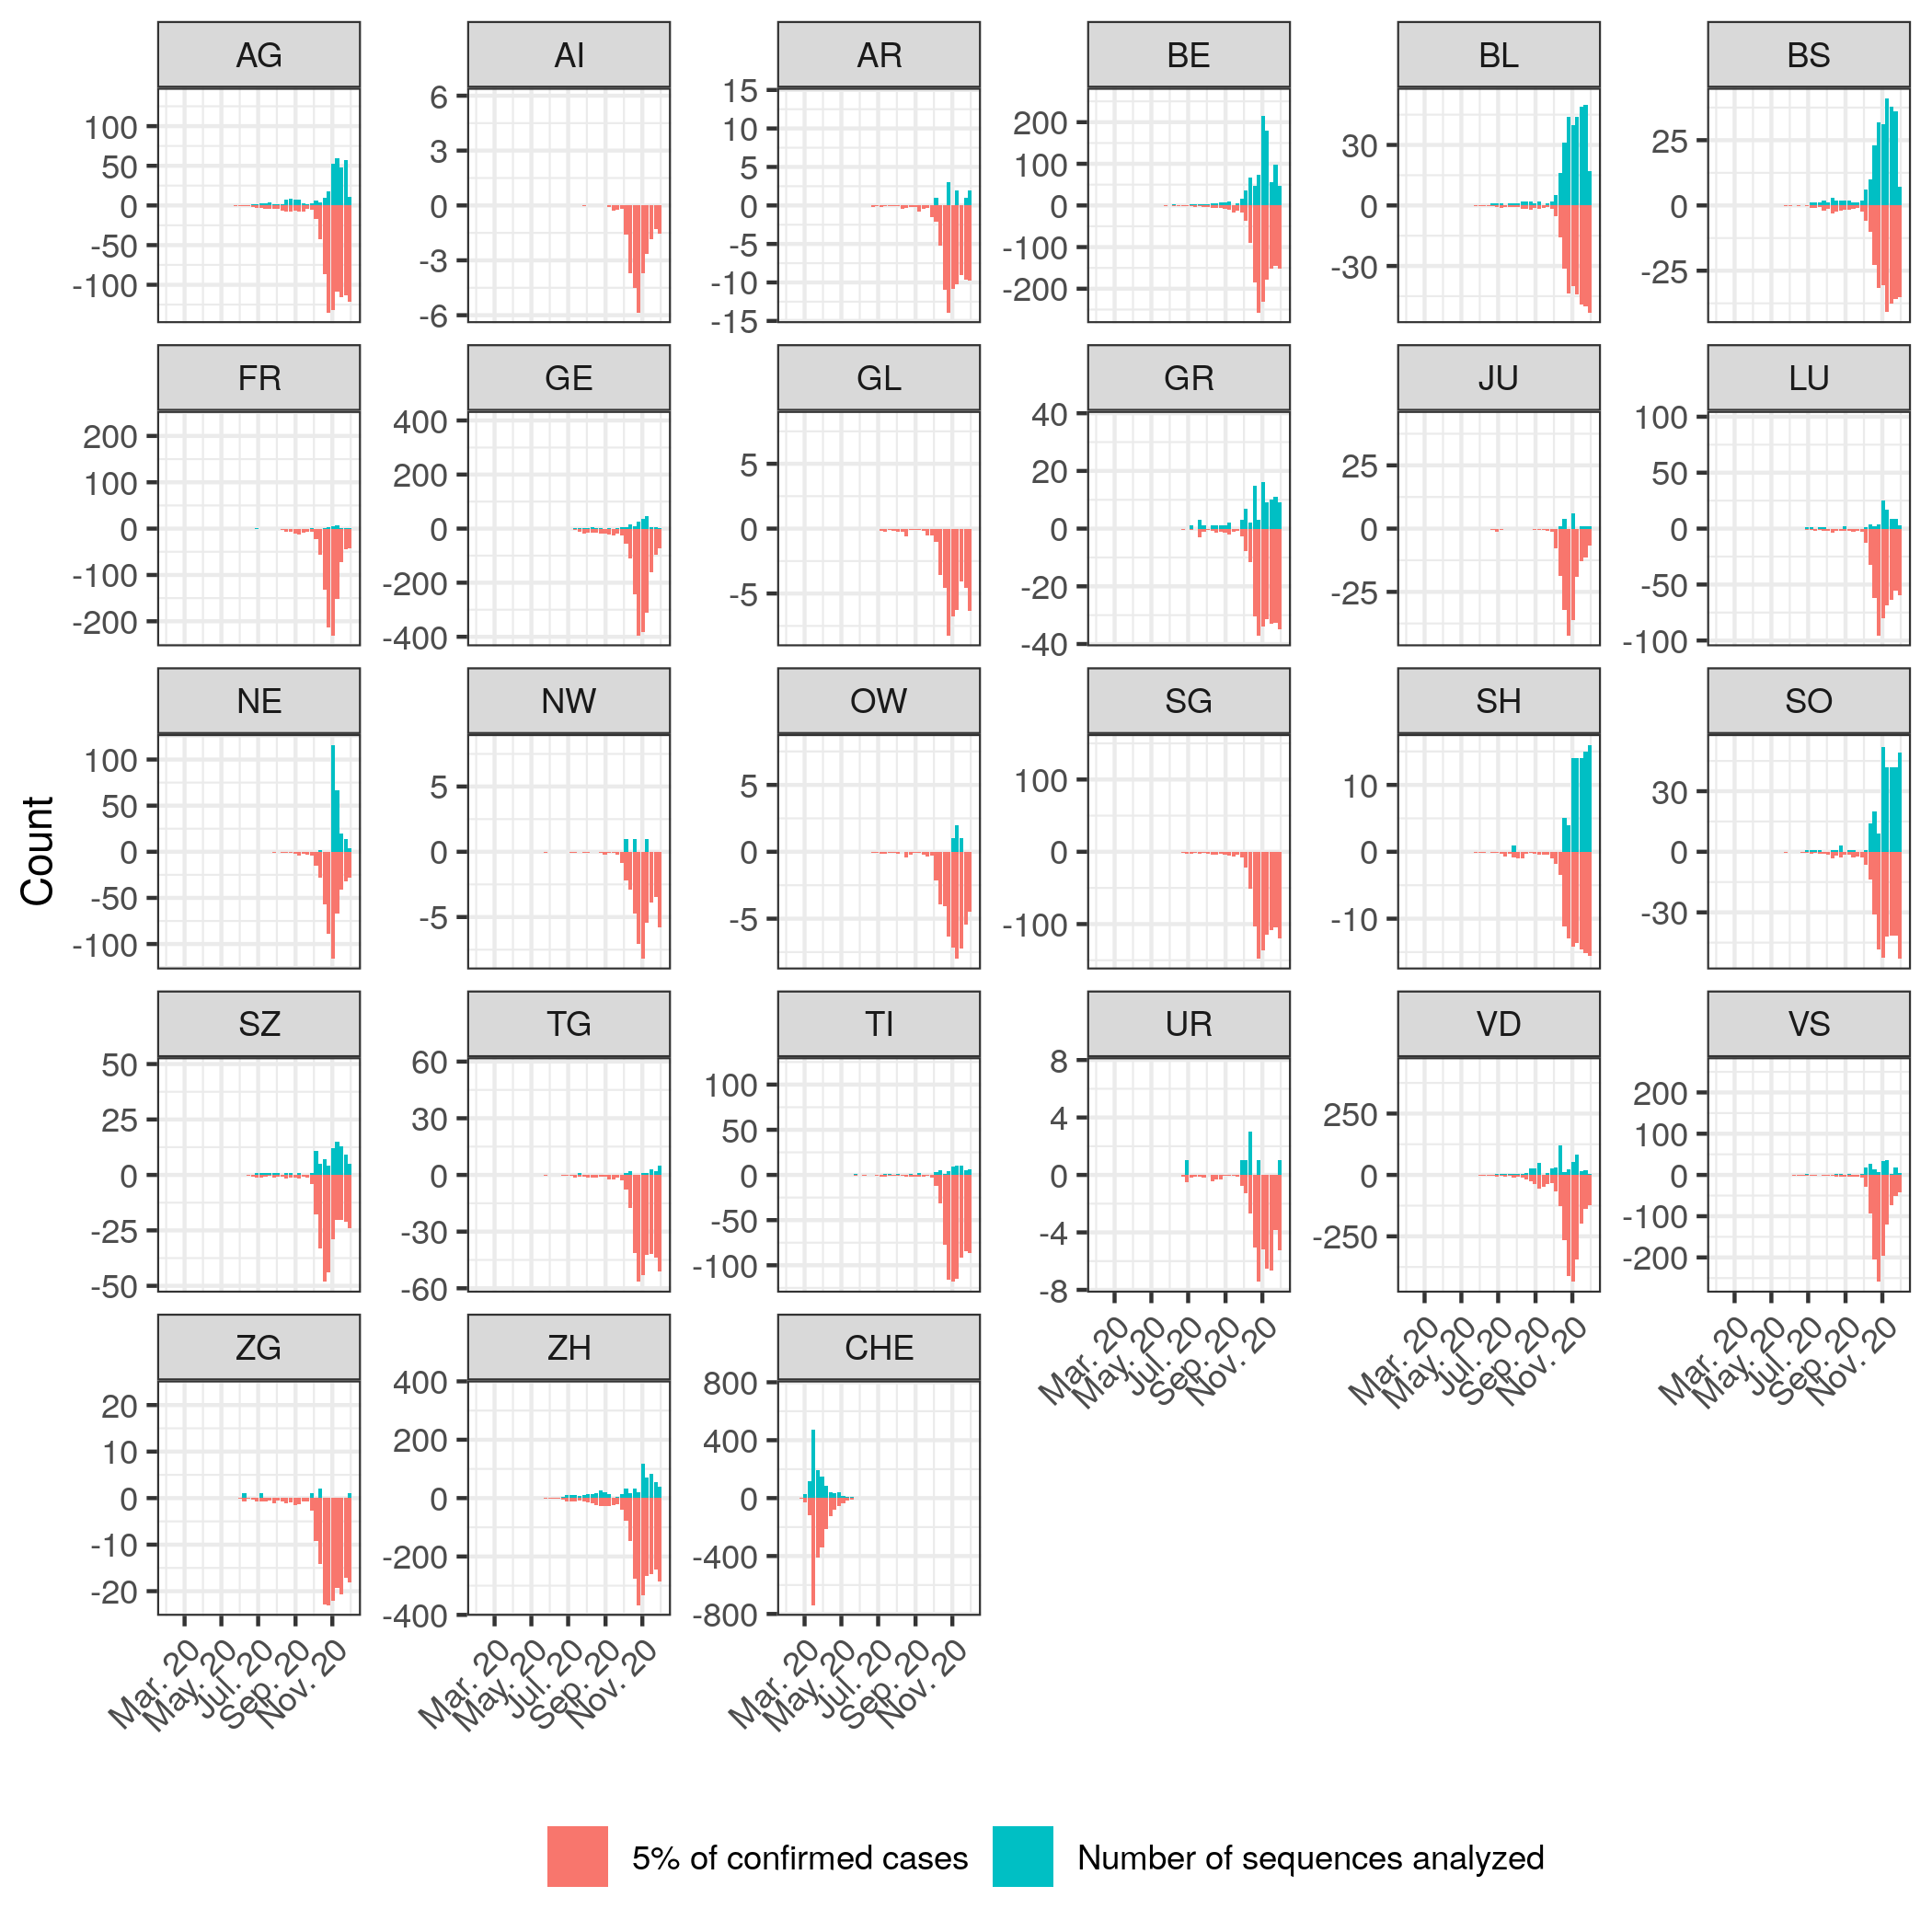
\includegraphics[width = 0.8\linewidth]{figures/CHE_downsampling.png}
\caption{Spatio-temporal representativeness of analyzed genome sequences. The mirror y-axis aims to contrast temporal trends in confirmed cases (red) versus analyzed sequences (blue); all values are positive counts. Facet titles are standard abbreviations for Swiss cantons. 'CHE' represents Swiss-wide cases and sequences, since case count reporting by canton began mid-May 2020.}  
\label{fig:downsampling_representativeness}
\end{figure}

\begin{figure}[h!]
\centering
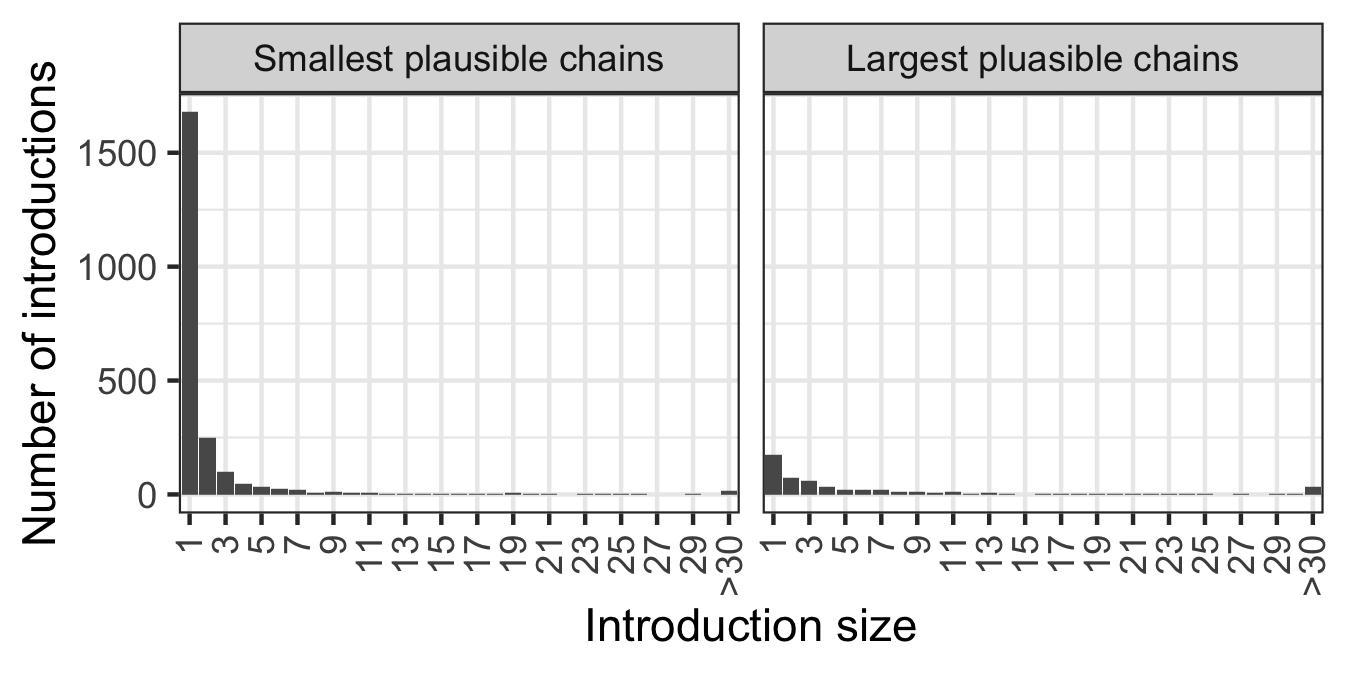
\includegraphics[width = 0.5\linewidth]{figures/chain_size_dist.png}
\caption{Size distribution of estimated introductions.}  
\label{fig:chain_size_dist}
\end{figure}

\begin{figure}[h!]
\centering
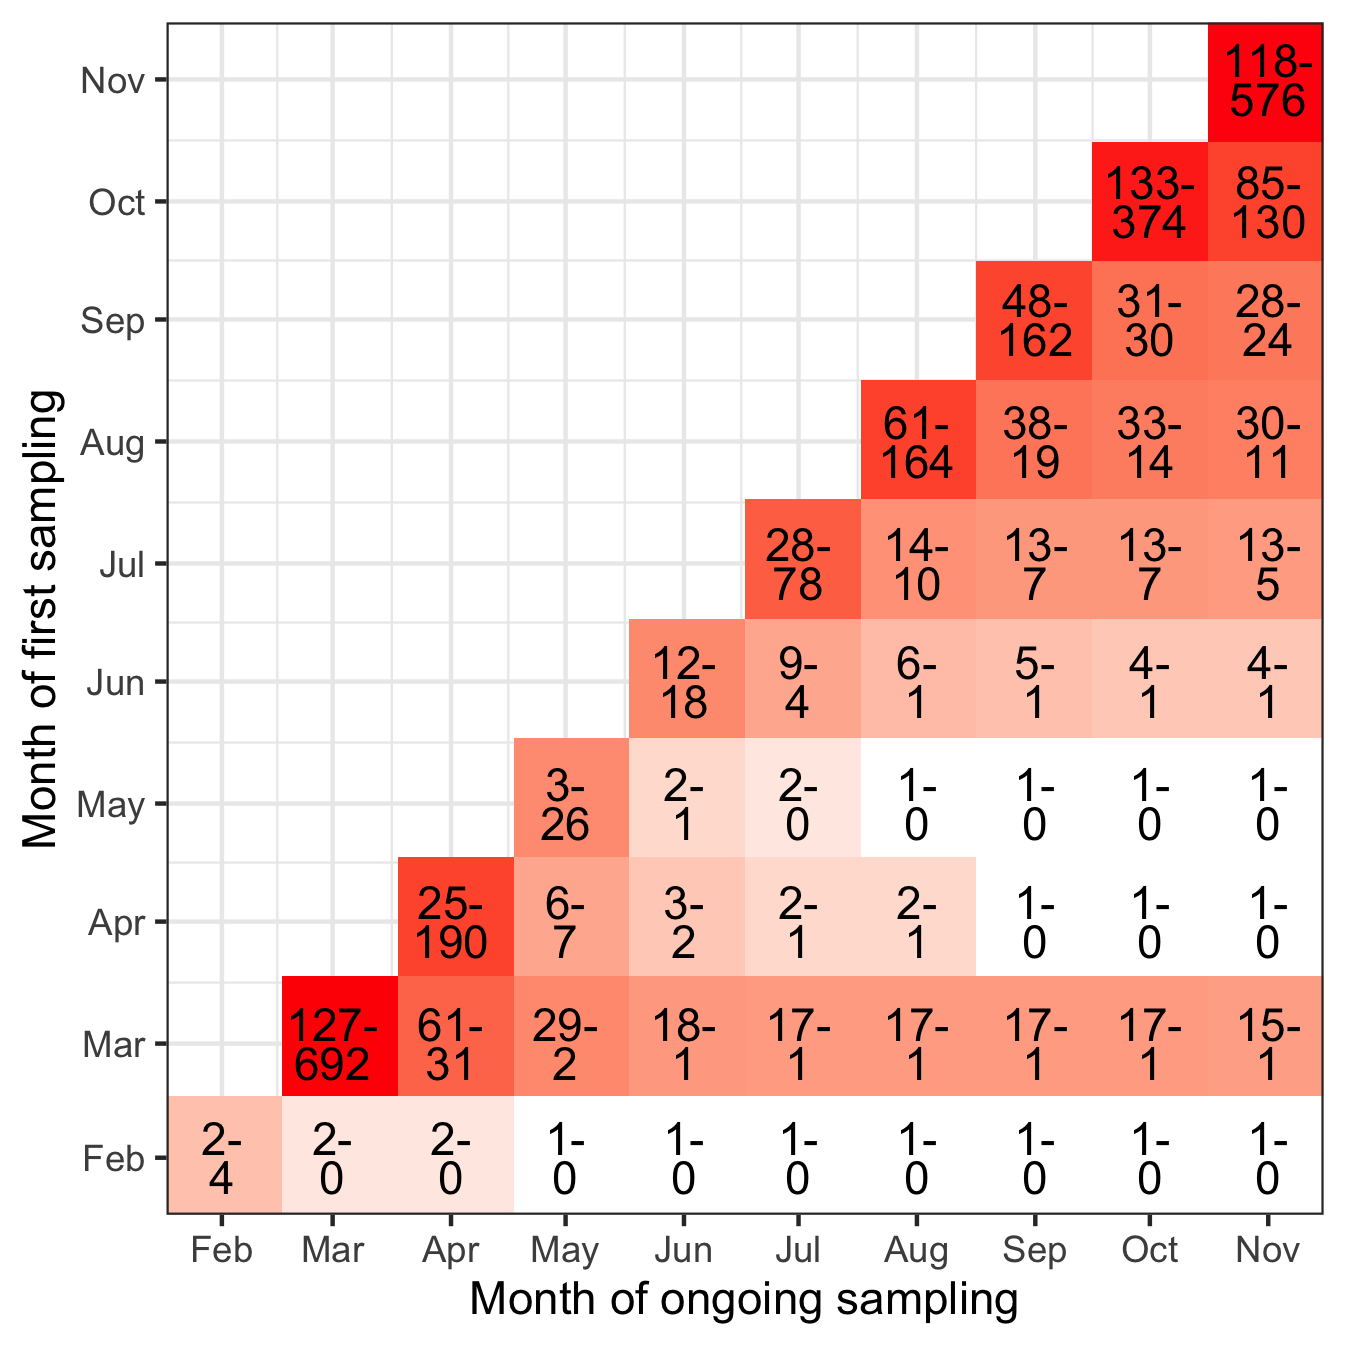
\includegraphics[width = 0.5\linewidth]{figures/chain_longevity_matrix.png}
\caption{Heatmap of the number of newly sampled introductions in Switzerland each month (diagonal entries) and the number continuing to persisting into each following month (off-diagonal entries). Introduction are counted once in the month they are first sampled (``Month of first sampling'') and one every following month (``Month of ongoing sampling'') until the date of the latest sample. The ranges are between two point estimates generated assuming either few or many introductions.}  
\label{fig:chain-longevity-matrix}
\end{figure}

\begin{figure}[h!]
\centering
\begin{subfigure}[b]{\textwidth}
\centering
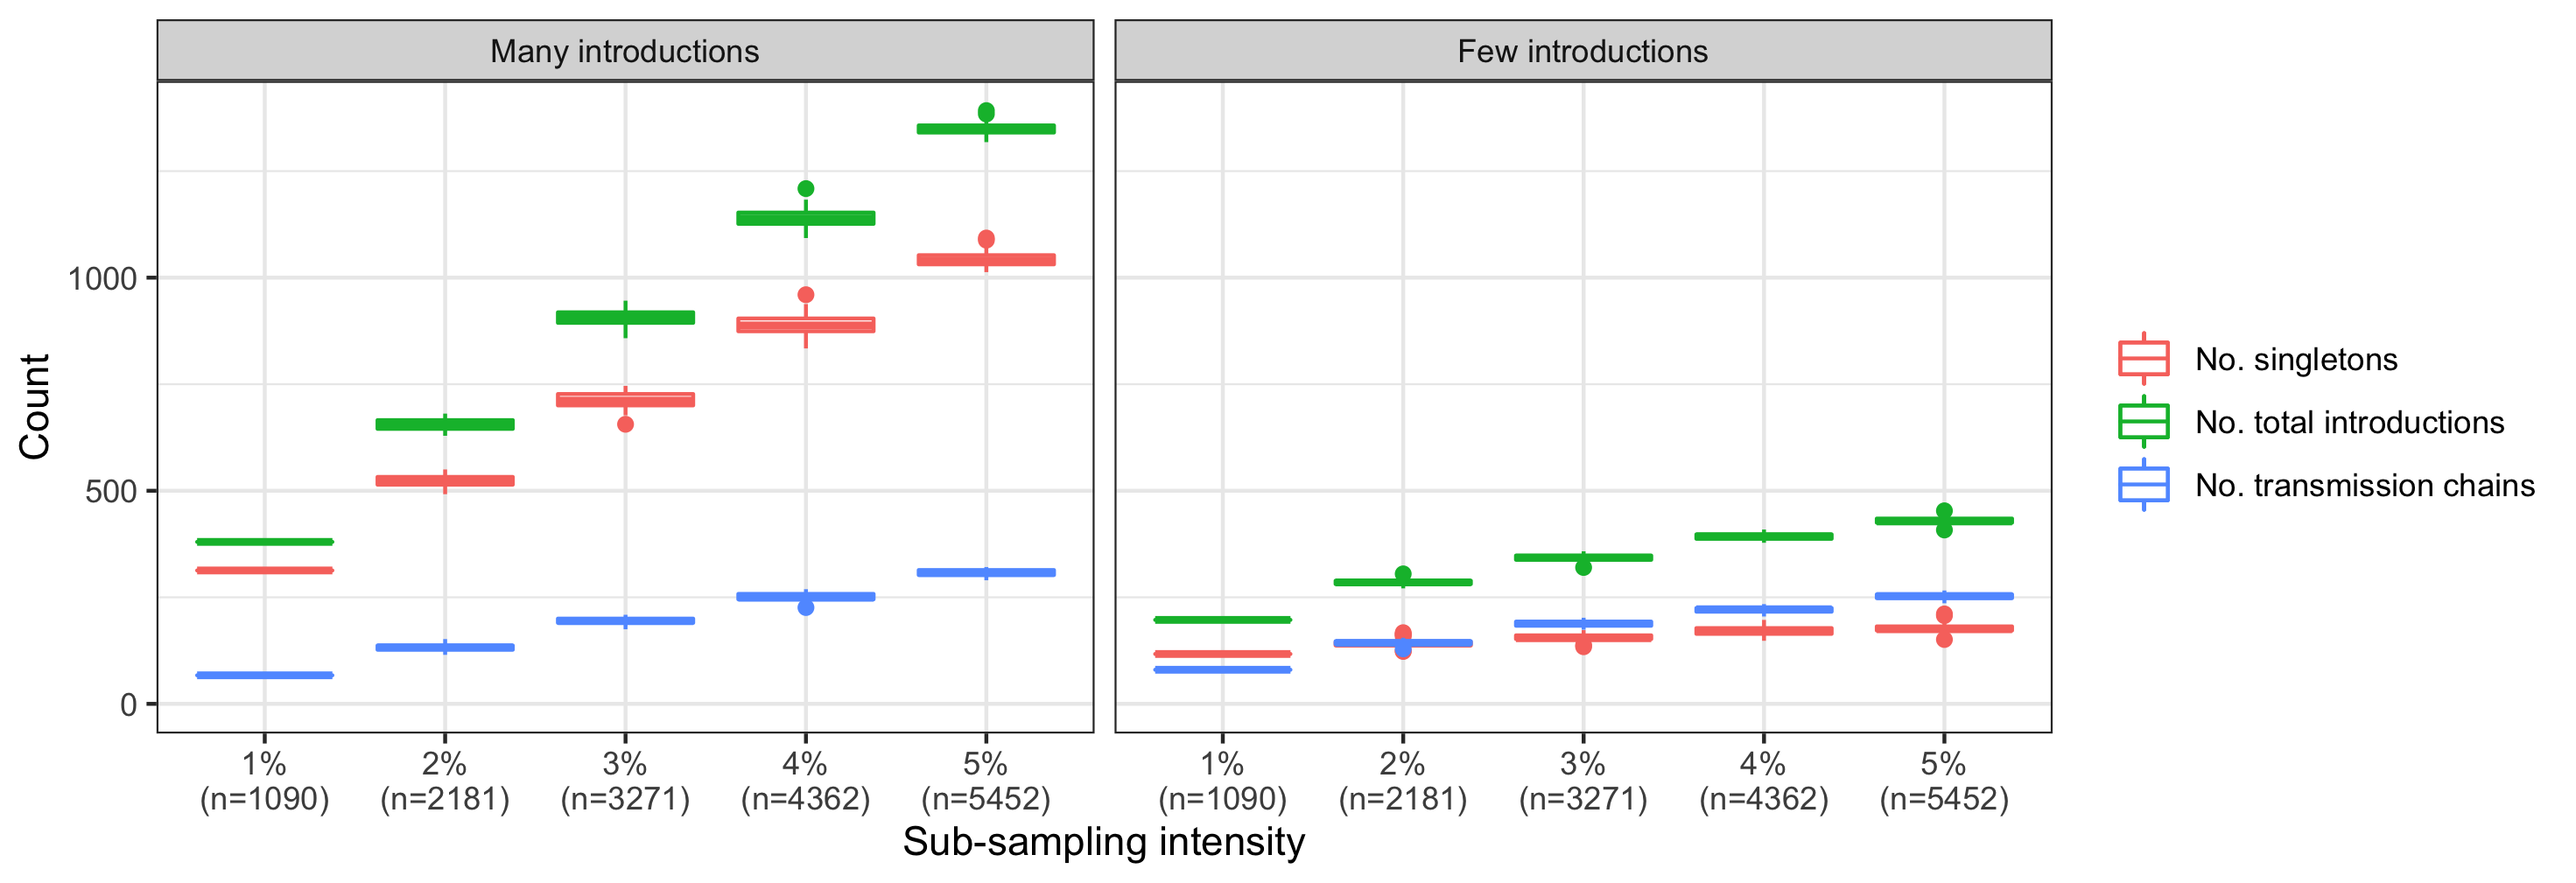
\includegraphics[width = 11.4cm]{figures/fig_SX_sensitivity_subsampling.png}
\caption{Estimated introductions by percent (or, n=number) of Swiss confirmed cases analyzed. No. = number. Each box plot is a summary over 50 random sub-samples.}  
\end{subfigure}

\begin{subfigure}[b]{0.9\textwidth}
\centering
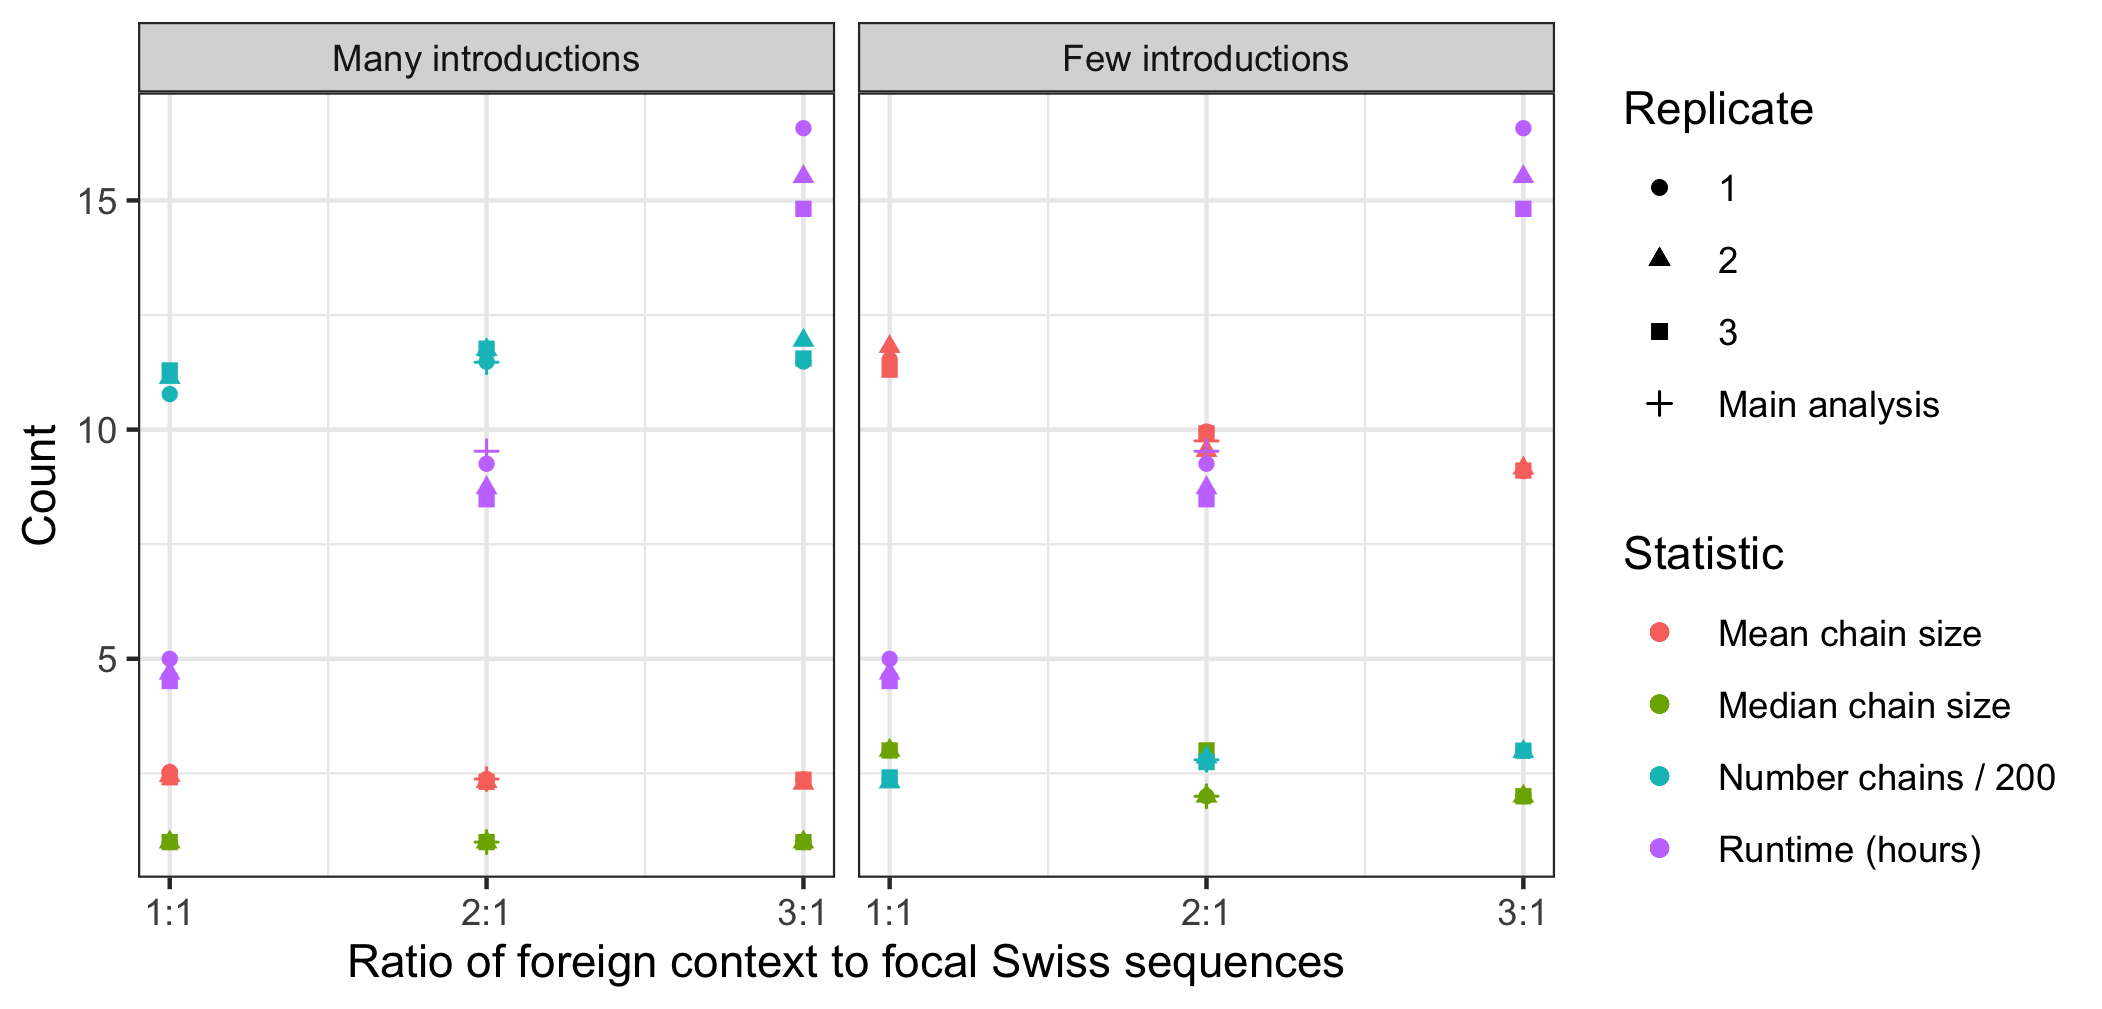
\includegraphics[width = 11.4cm]{figures/fig_SX_sensitivity_context_set_size.png}
\caption{Summary statistics about introductions by ratio of foreign context to focal Swiss sequences.}  
\end{subfigure}

\begin{subfigure}[b]{0.9\textwidth}
\centering
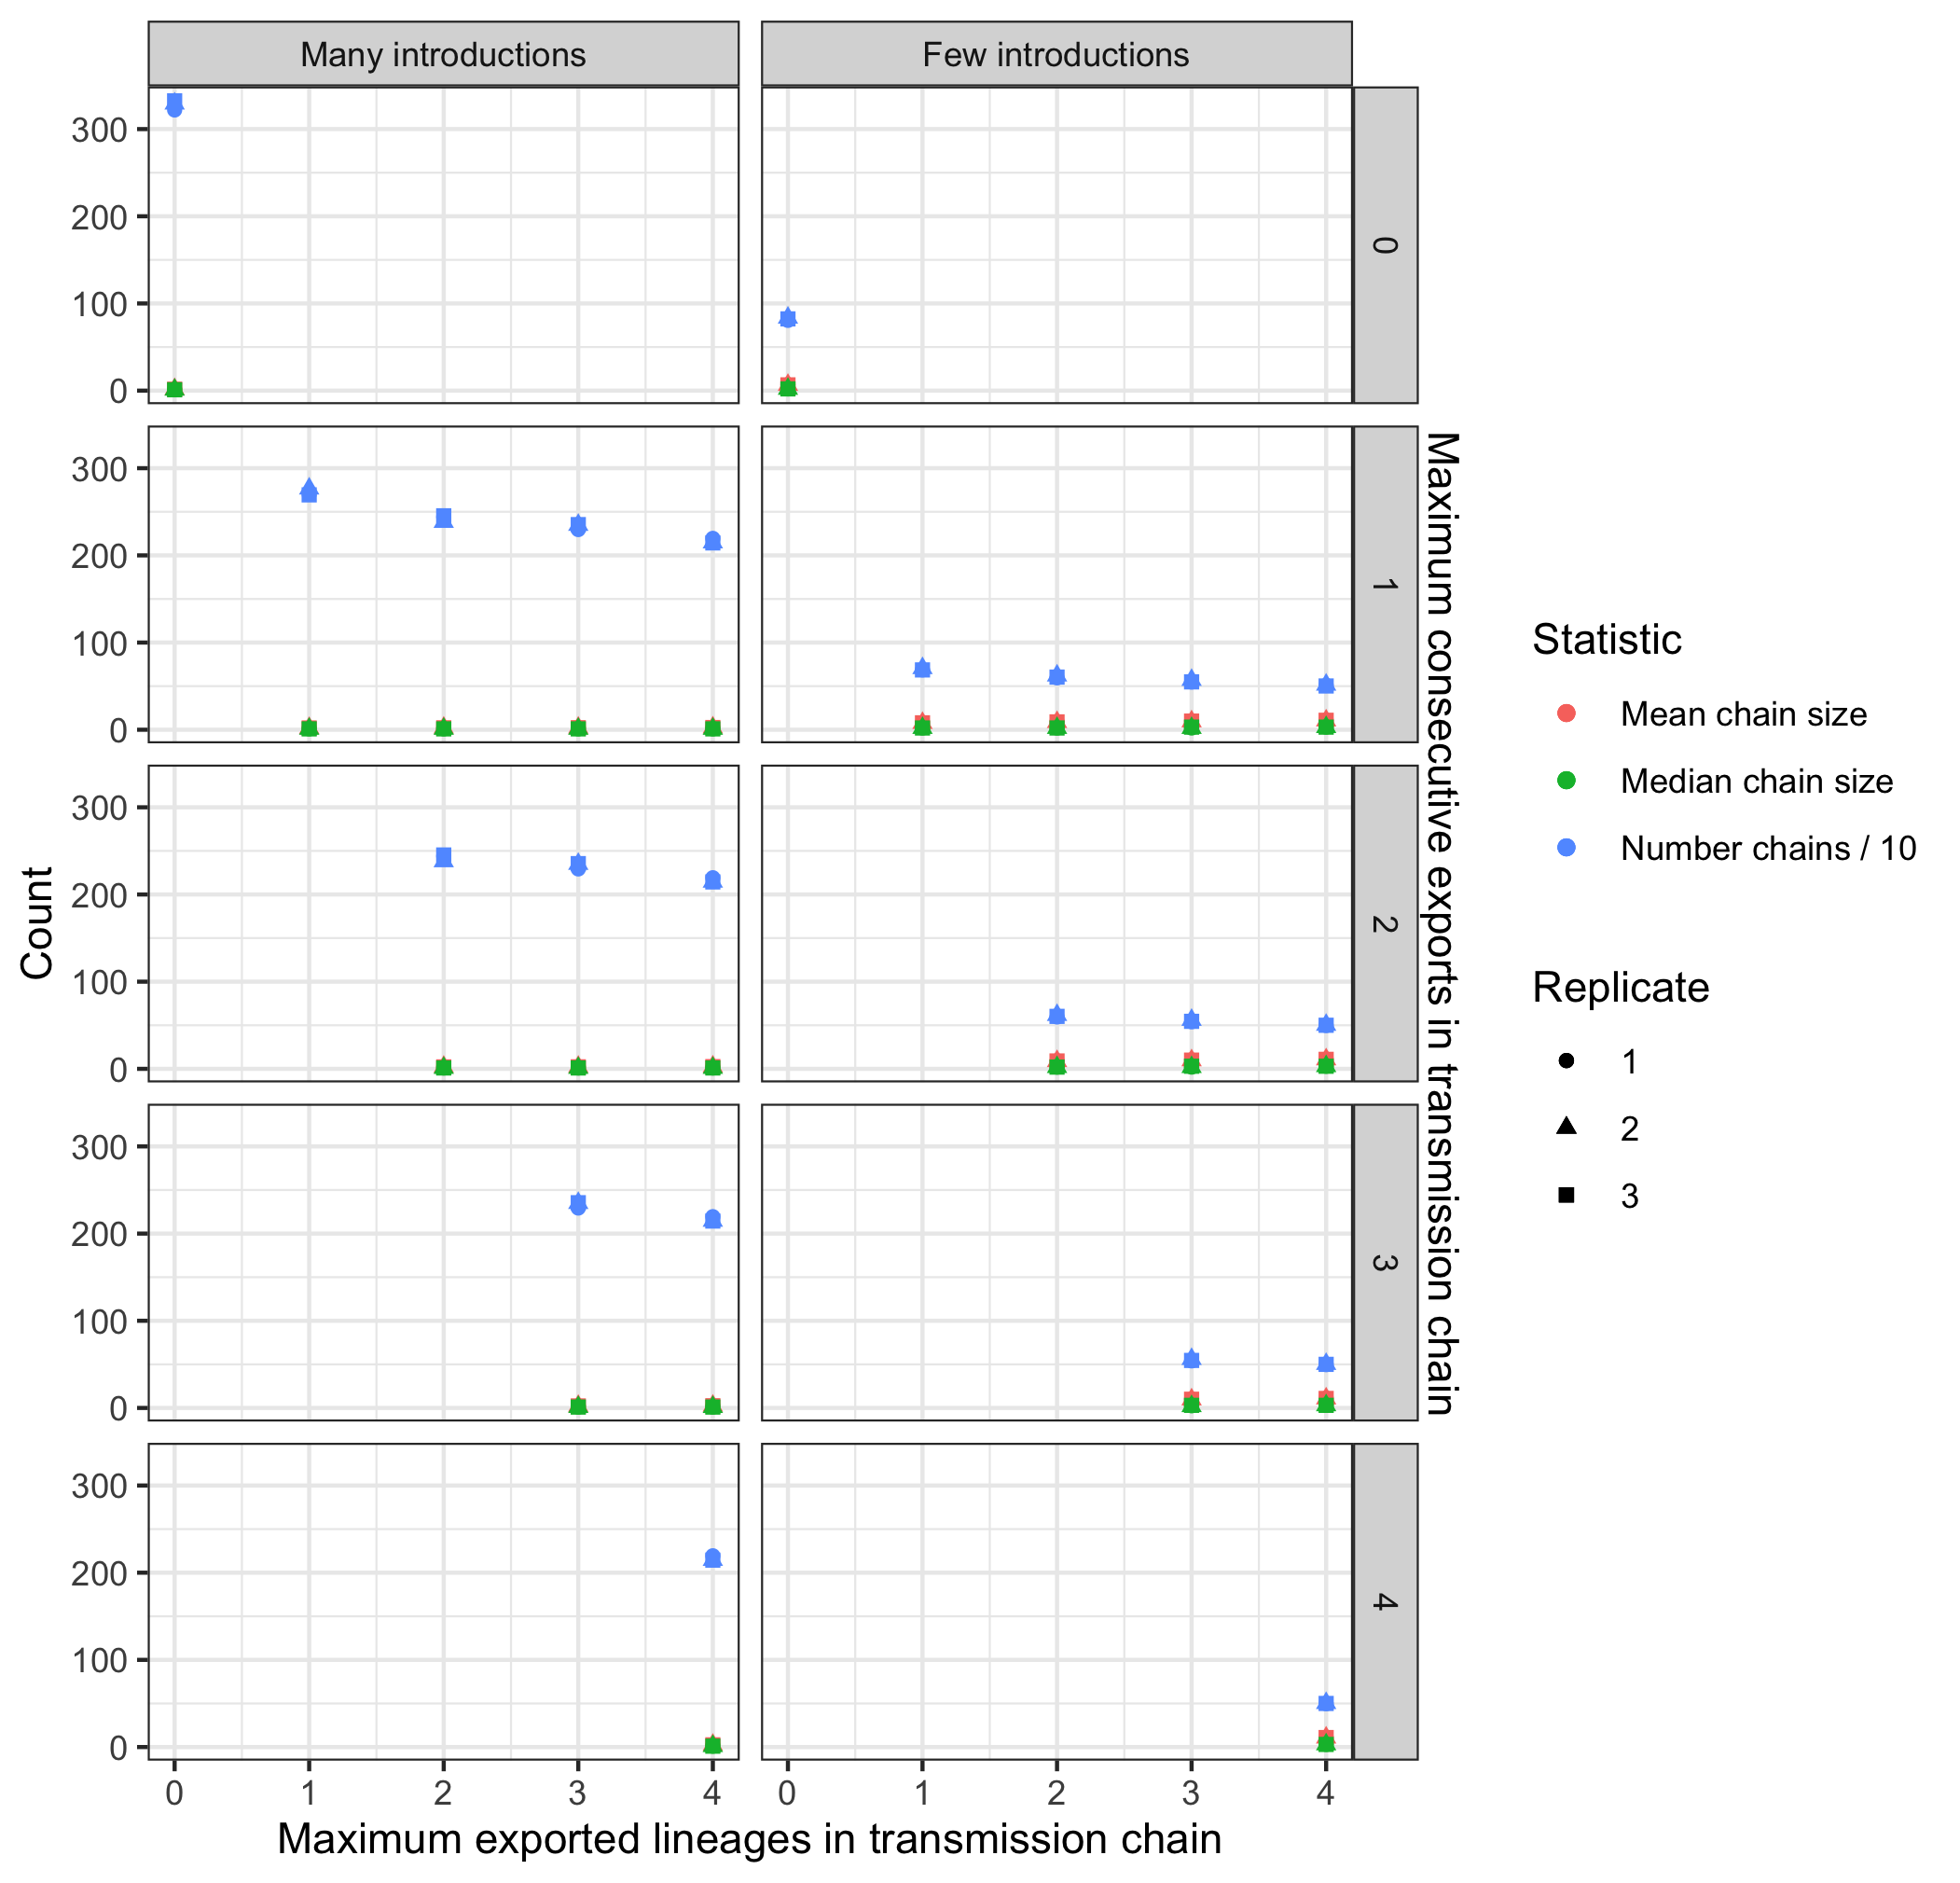
\includegraphics[width = 11.4cm]{figures/fig_SX_sensitivity_chain_defn.png}
\caption{Summary statistics about introductions and pipeline runtime by different heuristic definitions of an introduction.}  
\end{subfigure}
\caption{Sensitivity analyses for the definition of an introduction. (a) shows sensitivity to number of focal sequences analyzed, (b) shows sensitivity to the ratio of foreign context to focal sequences analyzed, and (c) shows sensitivity to the heuristic thresholds used to define an introduction given a tree. All statistics were generated under two different polytomy assumptions giving rise to either many or few introductions.}
\label{fig:sensitivity_figs}
\end{figure}

\begin{figure}[h!]
    \centering
    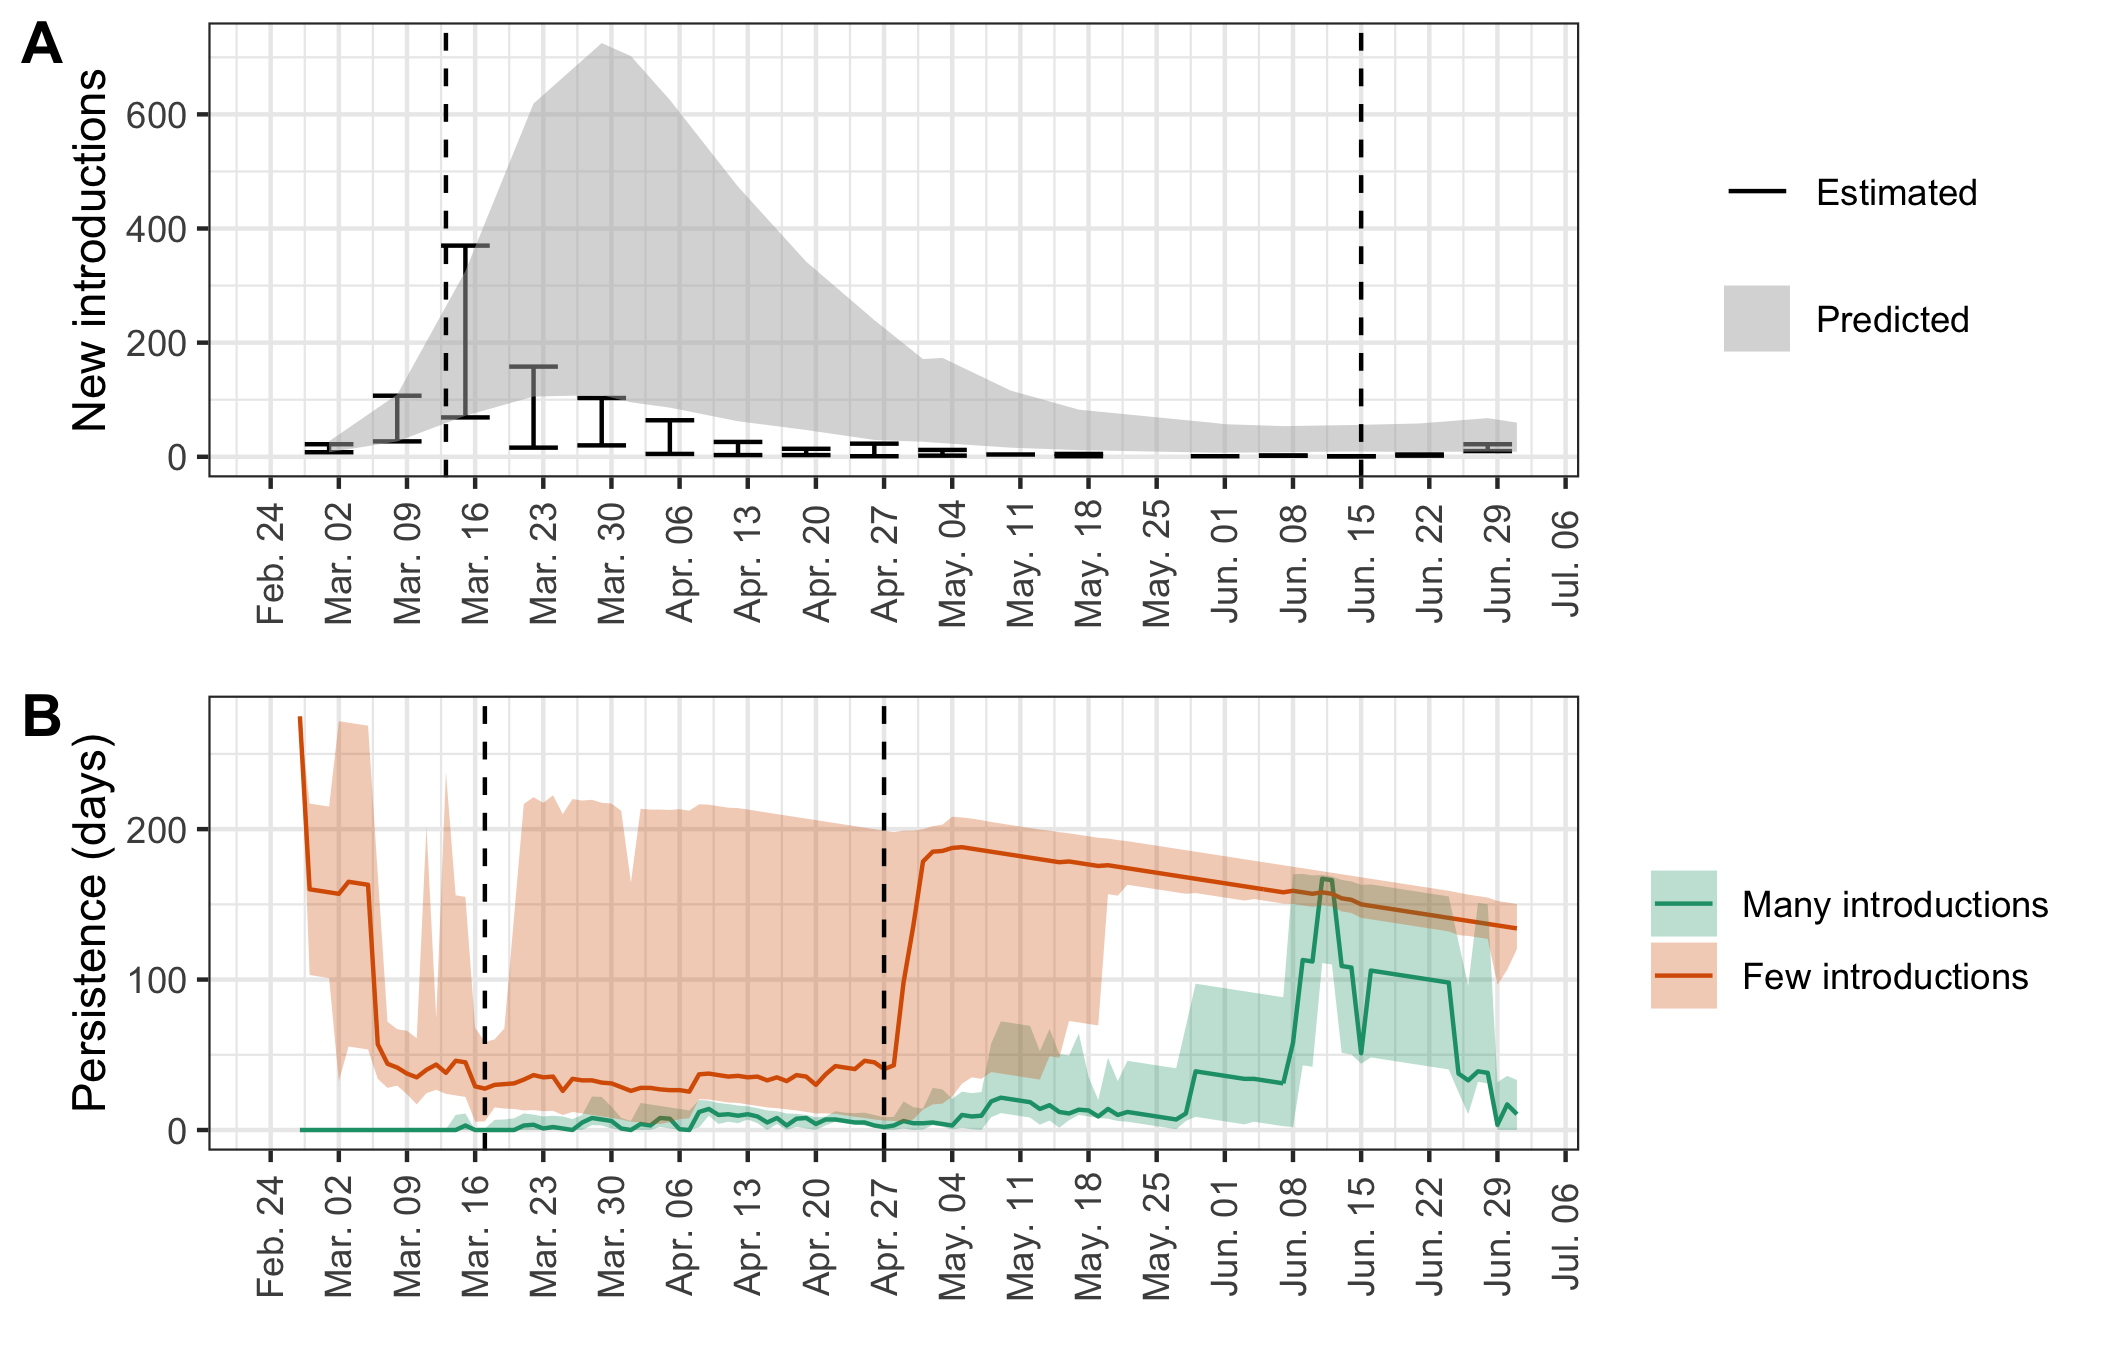
\includegraphics[width=\linewidth]{figures/introductions_and_persistence_v2.png}
    \caption{Introductions into Switzerland and their persistence around the time of the Swiss border closures and partial lockdown. (A) compares weekly introductions estimated from the genome data (bars) with predicted introductions based on case counts in Italy, France, Germany, and Austria (shaded area). The shaded area was fit to the genome-based estimates prior to the dashed line on 13 Mar 2020, the date of Swiss border closures, and the model fit is extrapolated after this date. (B) shows how the persistence of estimated introductions changed around the time of the Swiss lockdown, which is also represented by dashed lines. Persistence is shown as the median time from each date until introductions circulating on that date are last sampled. The shaded region shows the interquartile range and the two different colors are for estimates generated from the two different plausible sets of introductions, few and many.}
    \label{fig:introductions_and_persistence_v2}
\end{figure}

% \begin{landscape}
\begin{figure}[h!]
\centering
\begin{subfigure}[b]{\textwidth}
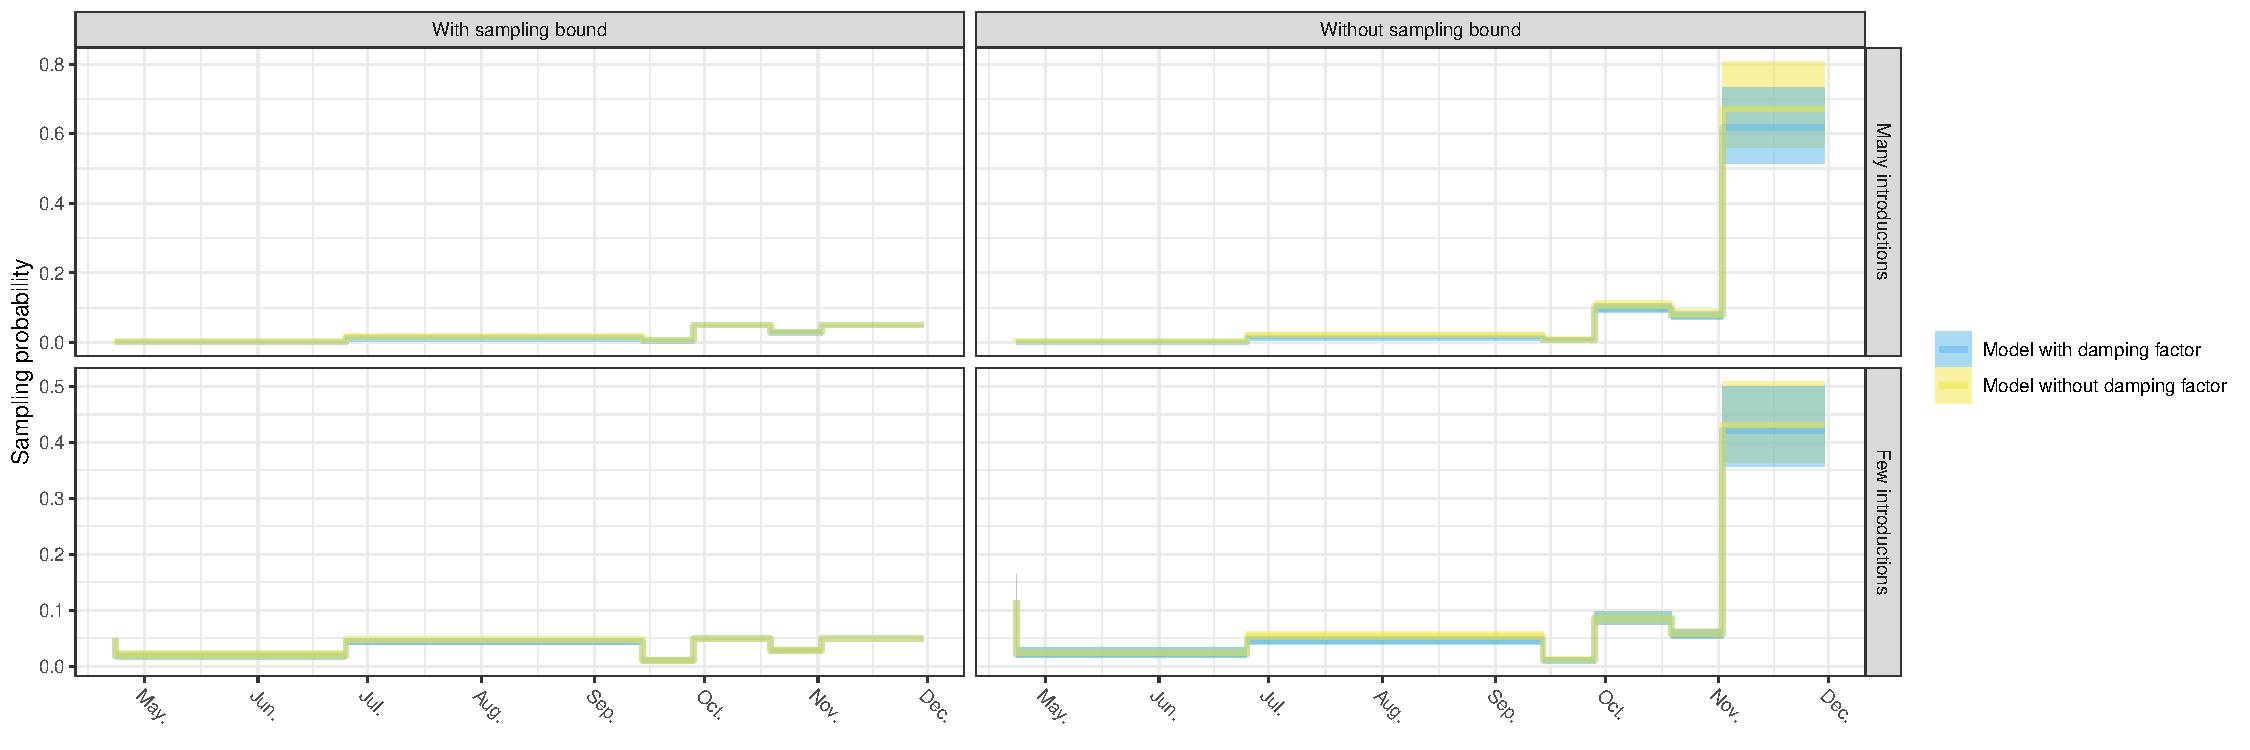
\includegraphics[width=\linewidth]{figures/CHE_sampProp.pdf}
\caption{Sampling probability in Switzerland.}
\end{subfigure}
\begin{subfigure}[b]{\textwidth}
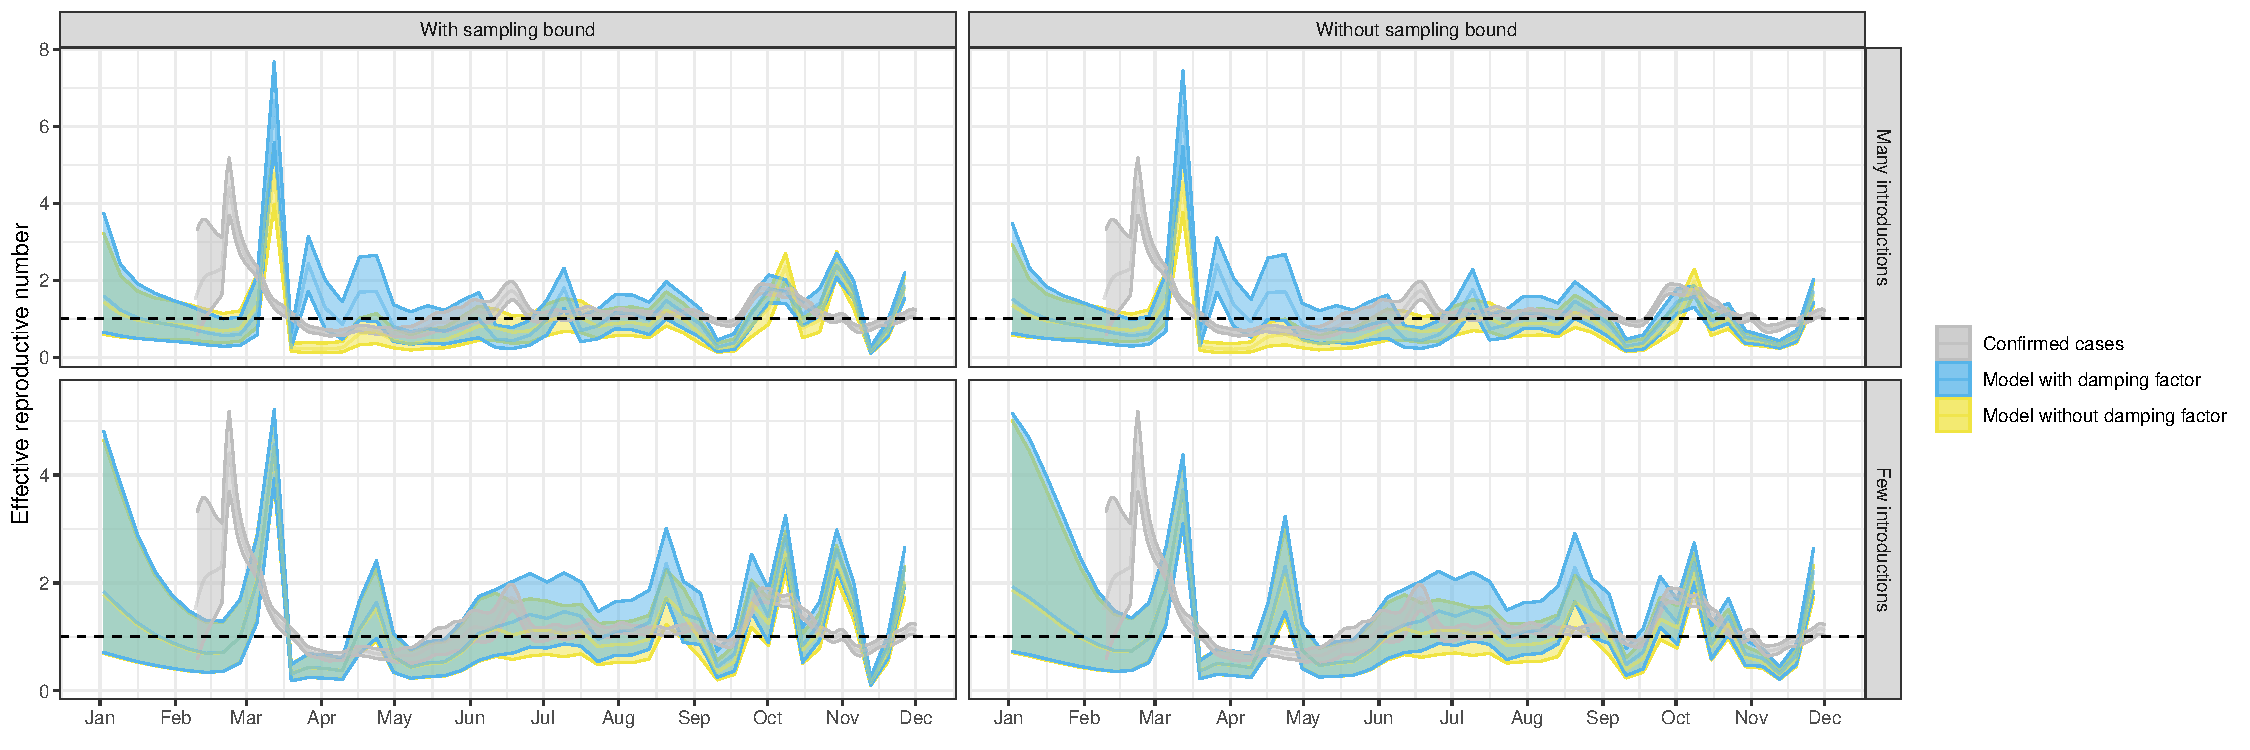
\includegraphics[width=\linewidth]{figures/CHE_Re.pdf}
\caption{Effective reproductive number in Switzerland.}
\end{subfigure}
\begin{subfigure}[b]{\textwidth}
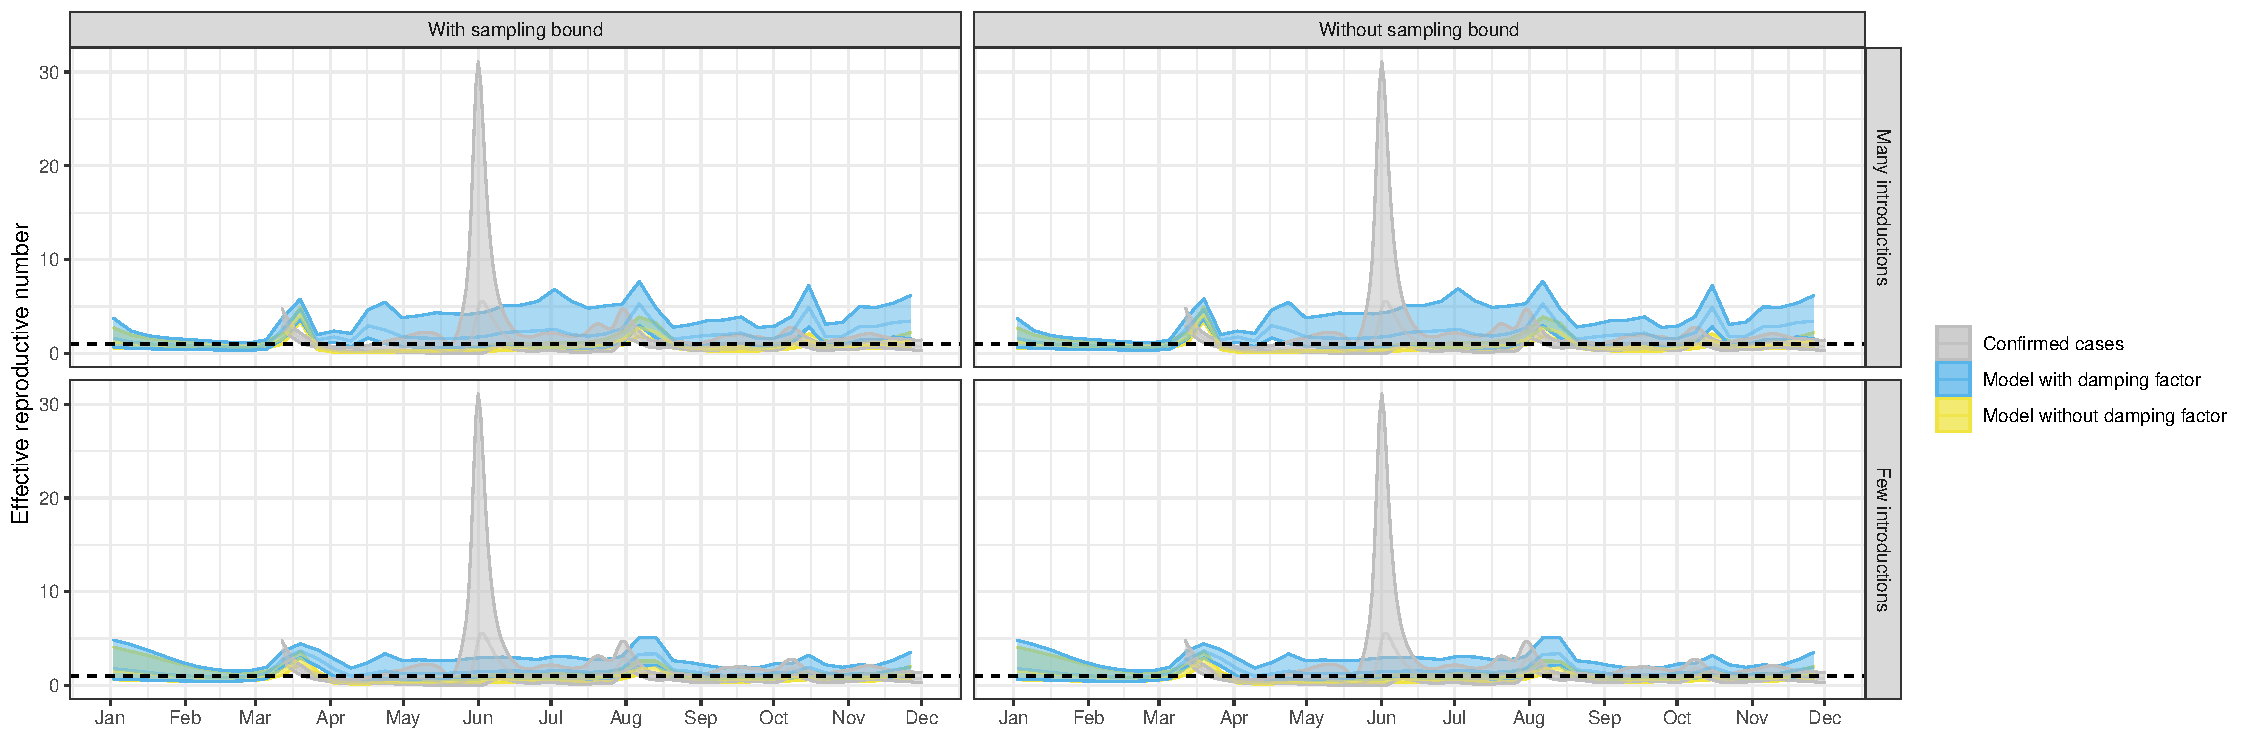
\includegraphics[width=\linewidth]{figures/NZL_Re.pdf}
\caption{Effective reproductive number in New Zealand.}
\end{subfigure}
\caption{Phylodynamic estimates for  (a) the sampling probability in Switzerland and the time-varying effective reproductive number $R_e$ in Switzerland (b) and New Zealand (c). $R_e$ estimates are overlaid on estimates generated from case count data \cite{huisman_re_preprint} in grey. Additionally, $R_e$ estimates from the models with a damping factor (pink) are the ``baseline'' $R_e$ before introduction-specific damping (i.e. before application of a damping factor once introductions are older than 2-days post sampling).}  
\label{fig:ReSampProbResults}
\end{figure}
% \end{landscape}
% Remember Re plot is now background Re (without contact tracing) and no longer the actual average Re

\begin{figure}[h!]
\centering
\begin{subfigure}[b]{0.7\textwidth}
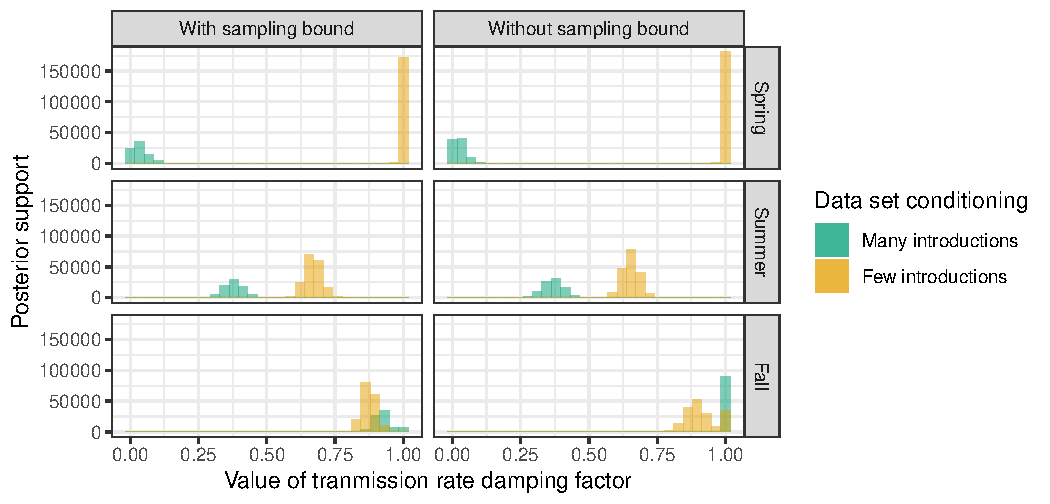
\includegraphics[width=\linewidth]{figures/CHE_contact_tracing_factor.pdf}
\caption{Damping factor in Switzerland.}
\end{subfigure}
\begin{subfigure}[b]{0.7\textwidth}
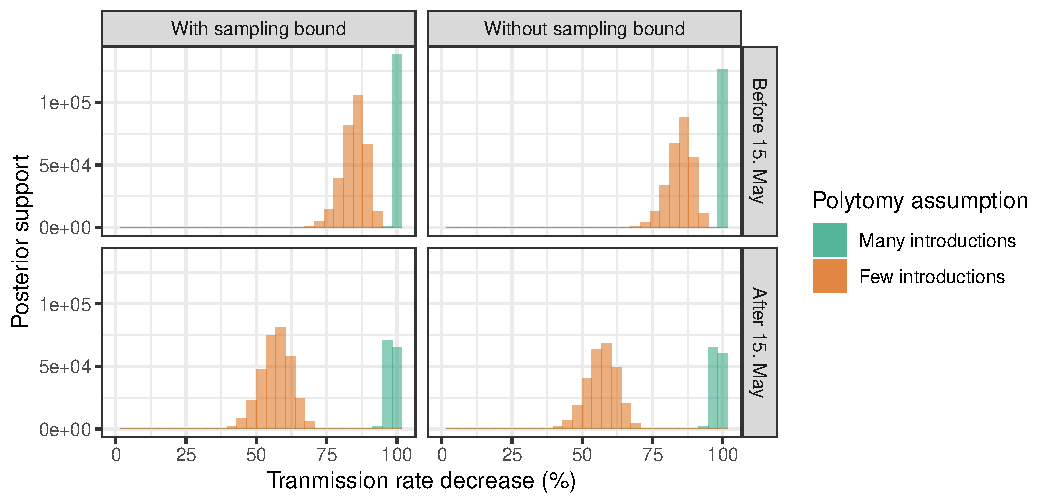
\includegraphics[width=\linewidth]{figures/NZL_contact_tracing_factor.pdf}
\caption{Damping factor in New Zealand.}
\end{subfigure}
\caption{Phylodynamic estimates for the damping factor in Switzerland and New Zealand in different time periods, conditioned on introductions defined using different polytomy assumptions and using different priors on the sampling probability.}  
\label{fig:DampingFactorResults}
\end{figure}
\newpage

\begin{landscape}
\begin{figure}[h!]
\centering
\begin{subfigure}[b]{0.65\textwidth}
\centering
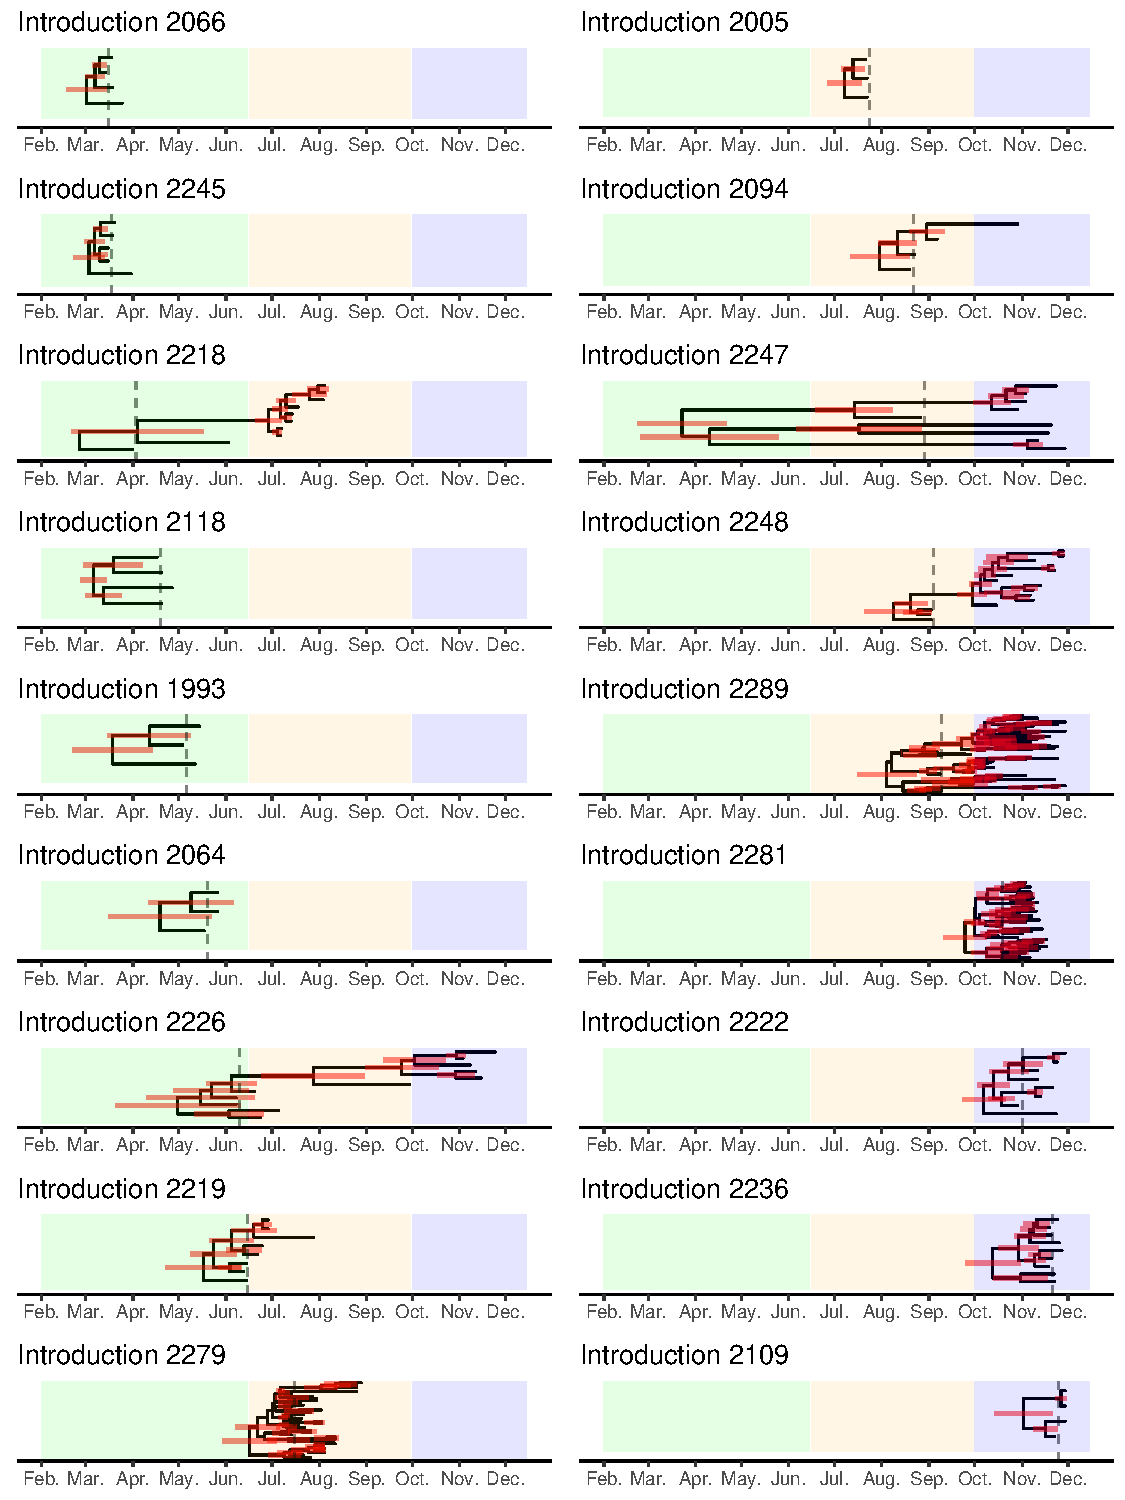
\includegraphics[width=0.75\linewidth]{figures/Re_skyline.max_chains.sampUB1.0.ctEst1.summary_trees.pdf}
\caption{Summary trees for introductions defined assuming many introductions.}
\end{subfigure}
\begin{subfigure}[b]{0.65\textwidth}
\centering
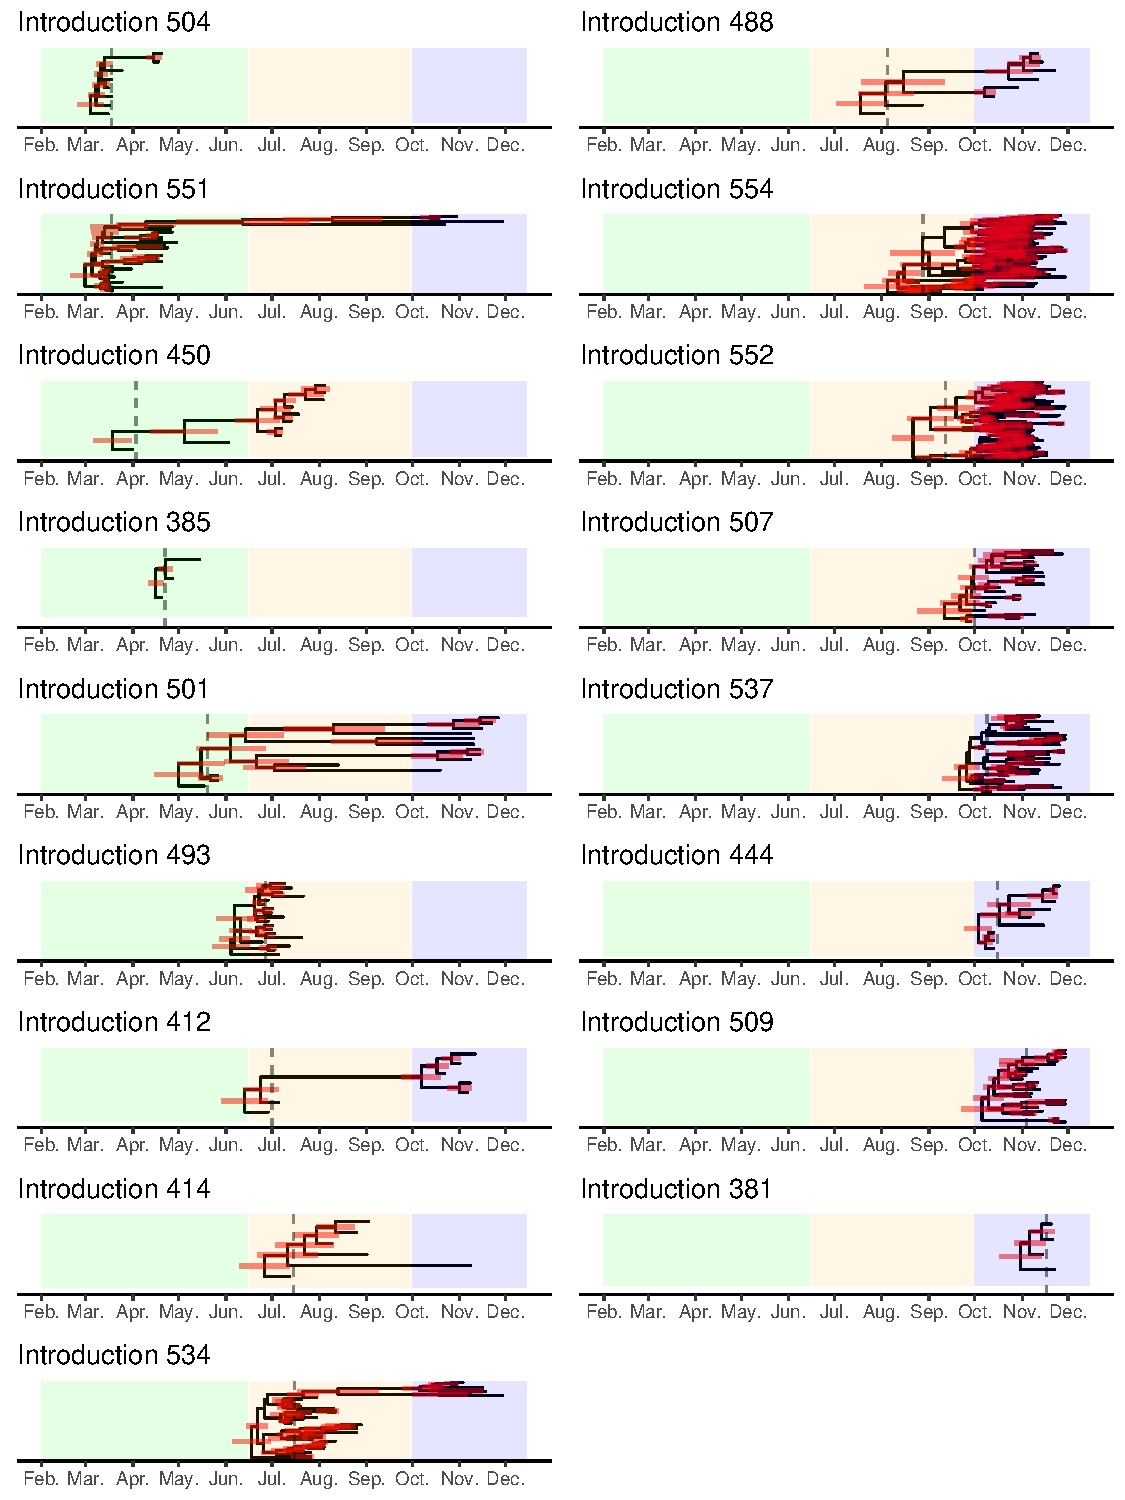
\includegraphics[width=0.75\linewidth]{figures/Re_skyline.min_chains.sampUB1.0.ctEst1.summary_trees.pdf}
\caption{Summary trees for introductions defined assuming few introductions.}
\end{subfigure}
\caption{Summary trees from the phylodynamic analysis for Switzerland. (a) and (b) show trees for introductions defined using different polytomy assumptions. The 50th and 95th percentile largest introductions among those first sampled each month are shown. The three color regions represent the Spring (green), Summer (orange) and Fall (blue) periods. The vertical dashed line shows the date at which the transmission rate can slow for each introduction - two days after the first sample date. The red bars show the 95\% highest posterior density uncertainty in node dates.}  
\label{fig:logged-chains}
\end{figure}
\end{landscape}
\newpage

\section{Supporting information tables}

\begin{table}[h!]
% \centering
\caption{Top 20 largest SARS-CoV-2 sequencing data contributors to GISAID in 2020 by submitting lab.}
\label{tab:seq-contributions}
\begin{tabular}{lll}
\hline
Submitting lab & Countries represented (ISO codes) & Number of sequences \\
\hline
Wellcome Sanger Institute for the COVID-19 Genomics UK (COG-UK) Consortium & GBR & 96441 \\ 
COVID-19 Genomics UK (COG-UK) Consortium & GBR & 71371 \\ 
Albertsen Lab, Department of Chemistry and Bioscience, Aalborg University, Denmark & DNK & 27936 \\ 
Houston Methodist Hospital & USA & 27409 \\ 
Pathogen Genomics Center, National Institute of Infectious Diseases & JPN; MMR & 19708 \\ 
Department of Biosystems Science and Engineering, ETH Zürich & CHE & 11357 \\ 
MDU-PHL & AUS; TLS & 10459 \\ 
TGen North & USA & 9491 \\ 
Wyoming Public Health Laboratory & USA & 9172 \\ 
Aalborg University & DNK & 8439 \\ 
SeqCOVID-SPAIN consortium/IBV(CSIC) & ESP & 8279 \\ 
Chan-Zuckerberg Biohub & USA & 7803 \\ 
BCCDC Public Health Laboratory & CAN & 7646 \\ 
Laboratoire de santé publique du Québec & CAN & 6914 \\ 
Andersen lab at Scripps Research & JOR; MEX; USA & 6258 \\ 
Utah Public Health Laboratory & USA & 5925 \\ 
MEPHI, Aix Marseille University & FRA & 5617 \\ 
Respiratory Virus Unit, Microbiology Services Colindale, Public Health England & GBR; UKR & 5142 \\ 
deCODE genetics & ISL & 5005 \\ 
Erasmus Medical Center & BEL; BHR; LUX; NLD; SUR & 4594 \\
\hline
\end{tabular}
\end{table}

\begin{table}[h!]
% \centering
\caption{Sampling proportion change-points for the phylodynamic analysis on Swiss data. The sampling proportion was modelled as a piece-wise-constant function in time, with the following change-points motivated by major shifts in the testing regime or genome sequencing intensity in Switzerland.}
\label{tab:CHE_samp_prob_change_dates}
\begin{tabular}{ll}
\hline
Start date & Description \\
\hline
23. Apr 2020 & All symptomatic individuals can get tested \\
25. Jun 2020 & Government pays for tests for symptomatic individuals \\
14. Sept 2020 & Genome sampling $<<$ 5\% of confirmed cases \\
28. Sept 2020 & Number of tests conducted and \% positivity dramatically increase, genome sampling also increases \\
19. Oct 2020 & Genome sampling $<<$ 5\% of confirmed cases again \\
11. Nov 2020 & Genome sampling improves again \\
\hline
\end{tabular}
\end{table}

\begin{table}[h!]
\caption{Contingency table for singleton introductions and transmission chains by time period assuming many (right) and few (left)  introductions.}
\label{tab:lockdown-contingency}
% latex table generated in R 4.0.5 by xtable 1.8-4 package
% Fri Sep  3 16:31:51 2021
\begin{tabular}{lcccc}
\hline
& Singleton & Transmission chain & Total \\ 
\hline
MRCA during lockdown & 533 &  91 & 624 \\ 
MRCA not during lockdown & 1209 & 461 & 1670 \\ 
Total & 1742 & 552 & 2294 \\ 
\hline
\end{tabular}

% latex table generated in R 4.0.5 by xtable 1.8-4 package
% Fri Sep  3 16:31:51 2021
\begin{tabular}{lcccc}
  \hline
 &  & Singleton & Transmission chain & Total \\ 
  \hline
1 & MRCA during lockdown &  47 &  28 &  75 \\ 
  2 & MRCA not during lockdown & 152 & 332 & 484 \\ 
  3 & Total & 199 & 360 & 559 \\ 
   \hline
\end{tabular}

\end{table}

% latex table generated in R 4.0.5 by xtable 1.8-4 package & modified manually
% Thu Aug 12 18:13:52 2021
\begin{longtable}[l]{cccP{4cm}c}
\caption{Summary of Pango lineages analyzed. If more than 50\% of the samples from a lineage in the full, quality-filtered dataset were Swiss, we aggregated them into the parent lineage. The percentage of Swiss samples in the final, aggregated lineage sets are given in column ``\% lineage Swiss''. Lineage aliases were also aggregated with their extended-form names. A separate phylogeny was constructed for each lineage analyzed.}
\label{tab:lineage-data-summary}
\hline
 & Lineage analyzed & No. Swiss samples analyzed & Lineages aggregated & \% lineage Swiss \\ 
\hline
1 & B.1.160 & 1347 & B.1.160, B.1.160.10, B.1.160.11, B.1.160.12, B.1.160.14, B.1.160.15, B.1.160.16, AB, B.1.160.19, B.1.160.20, B.1.160.22, B.1.160.26, B.1.160.29, B.1.160.30, B.1.160.31, B.1.160.32, B.1.160.9, B.1.160.16.1, AB.1 & 19.00 \\ 
  2 & B.1.177 & 1260 & B.1.177, B.1.177.23, B.1.177.28, B.1.177.43, B.1.177.44, B.1.177.71 & 4.80 \\ 
  3 & B.1 & 930 & B.1, B.1.214.2 & 2.20 \\ 
  4 & B.1.1 & 655 & B.1.1, B.1.1.144, B.1.1.327, B.1.1.39, AQ, B.1.1.524 & 3.10 \\ 
  5 & B.1.221 & 176 & B.1.221 & 8.10 \\ 
  6 & B.1.1.70 & 108 & B.1.1.70, AP & 15.00 \\ 
  7 & B.1.416.1 & 105 & B.1.416.1 & 45.00 \\ 
  8 & B.1.258 & 101 & B.1.258 & 4.40 \\ 
  9 & B.1.367 &  60 & B.1.367 & 10.00 \\ 
  10 & B.1.236 &  59 & B.1.236 & 33.00 \\ 
  11 & B.1.1.1.35 &  53 & B.1.1.1.35, C.35 & 13.00 \\ 
  12 & B.1.36.1 &  47 & B.1.36.1 & 35.00 \\ 
  13 & B.1.128 &  31 & B.1.128 & 3.30 \\ 
  14 & B.1.93 &  31 & B.1.93 & 3.30 \\ 
  15 & B.1.1.277 &  27 & B.1.1.277, K & 5.80 \\ 
  16 & B.1.1.47 &  24 & B.1.1.47 & 32.00 \\ 
  17 & B.1.1.269 &  19 & B.1.1.269 & 5.00 \\ 
  18 & B.1.1.1.36 &  16 & B.1.1.1.36, C.36, B.1.1.1.36.2, C.36.2 & 9.30 \\ 
  19 & B.1.1.10 &  16 & B.1.1.10, L & 2.70 \\ 
  20 & B.1.1.7 &  16 & B.1.1.7, Q & 0.85 \\ 
  21 & B.1.1.1 &  15 & B.1.1.1, C, B.1.1.1.5, C.5 & 0.86 \\ 
  22 & B.1.1.189 &  15 & B.1.1.189 & 12.00 \\ 
  23 & B.1.146 &  15 & B.1.146 & 30.00 \\ 
  24 & B.1.1.232 &  14 & B.1.1.232, AK & 3.10 \\ 
  25 & B &  11 & B & 0.44 \\ 
  26 & B.1.1.153 &  11 & B.1.1.153 & 6.50 \\ 
  27 & B.1.1.305 &  11 & B.1.1.305, AF, B.1.1.305.1, AF.1 & 8.40 \\ 
  28 & B.1.1.372 &  11 & B.1.1.372 & 0.95 \\ 
  29 & B.1.177.75 &  11 & B.1.177.75 & 12.00 \\ 
  30 & B.1.177.77 &  11 & B.1.177.77 & 6.10 \\ 
  31 & B.1.1.200.1 &  10 & B.1.1.200.1, AN.1 & 33.00 \\ 
  32 & B.1.147 &  10 & B.1.147 & 0.84 \\ 
  33 & B.1.177.81 &  10 & B.1.177.81 & 1.80 \\ 
  34 & B.1.1.37 &   9 & B.1.1.37 & 0.42 \\ 
  35 & B.1.177.33 &   8 & B.1.177.33 & 4.50 \\ 
  36 & B.1.36 &   8 & B.1.36 & 0.80 \\ 
  37 & B.1.509 &   8 & B.1.509 & 2.30 \\ 
  38 & B.1.1.433 &   7 & B.1.1.433 & 7.80 \\ 
  39 & B.1.1.521 &   7 & B.1.1.521 & 19.00 \\ 
  40 & B.1.36.17 &   7 & B.1.36.17 & 1.20 \\ 
  41 & B.1.8 &   7 & B.1.8 & 1.80 \\ 
  42 & B.1.91 &   7 & B.1.91 & 1.60 \\ 
  43 & B.1.177.51 &   6 & B.1.177.51 & 20.00 \\ 
  44 & B.1.258.17 &   6 & B.1.258.17 & 1.40 \\ 
  45 & B.1.467 &   6 & B.1.467 & 33.00 \\ 
  46 & B.1.1.242 &   5 & B.1.1.242 & 35.00 \\ 
  47 & B.1.1.58 &   5 & B.1.1.58 & 14.00 \\ 
  48 & B.1.177.83 &   5 & B.1.177.83 & 7.80 \\ 
  49 & B.1.177.85 &   5 & B.1.177.85 & 11.00 \\ 
  50 & B.1.535 &   5 & B.1.535 & 0.59 \\ 
  51 & B.40 &   5 & B.40 & 0.23 \\ 
  52 & B.1.1.218 &   4 & B.1.1.218 & 5.20 \\ 
  53 & B.1.1.241 &   4 & B.1.1.241, AH & 4.20 \\ 
  54 & B.1.1.428 &   4 & B.1.1.428 & 50.00 \\ 
  55 & B.1.1.464 &   4 & B.1.1.464, AW & 1.20 \\ 
  56 & B.1.258.14 &   4 & B.1.258.14 & 11.00 \\ 
  57 & B.1.356 &   4 & B.1.356 & 0.82 \\ 
  58 & A &   3 & A & 0.15 \\ 
  59 & B.1.1.170 &   3 & B.1.1.170 & 2.60 \\ 
  60 & B.1.1.231.1 &   3 & B.1.1.231.1, AL.1 & 0.34 \\ 
  61 & B.1.1.297 &   3 & B.1.1.297, AG & 1.90 \\ 
  62 & B.1.1.317 &   3 & B.1.1.317, AS & 2.10 \\ 
  63 & B.1.1.371 &   3 & B.1.1.371 & 6.20 \\ 
  64 & B.1.177.52 &   3 & B.1.177.52, Y & 2.80 \\ 
  65 & B.1.177.53 &   3 & B.1.177.53, W & 3.60 \\ 
  66 & B.1.389 &   3 & B.1.389 & 1.50 \\ 
  67 & B.1.474 &   3 & B.1.474 & 14.00 \\ 
  68 & B.1.480 &   3 & B.1.480 & 4.30 \\ 
  69 & B.1.9.5 &   3 & B.1.9.5 & 11.00 \\ 
  70 & B.11 &   3 & B.11 & 1.80 \\ 
  71 & B.3 &   3 & B.3 & 0.37 \\ 
  72 & A.2 &   2 & A.2 & 0.22 \\ 
  73 & B.1.1.219 &   2 & B.1.1.219 & 1.60 \\ 
  74 & B.1.1.243 &   2 & B.1.1.243 & 4.20 \\ 
  75 & B.1.1.33 &   2 & B.1.1.33, N & 0.11 \\ 
  76 & B.1.1.44 &   2 & B.1.1.44 & 0.58 \\ 
  77 & B.1.1.50 &   2 & B.1.1.50 & 1.20 \\ 
  78 & B.1.160.28 &   2 & B.1.160.28 & 1.40 \\ 
  79 & B.1.177.15 &   2 & B.1.177.15, AA & 0.21 \\ 
  80 & B.1.177.32 &   2 & B.1.177.32 & 1.10 \\ 
  81 & B.1.177.53.1 &   2 & B.1.177.53.1, W.1 & 7.70 \\ 
  82 & B.1.177.55 &   2 & B.1.177.55 & 0.87 \\ 
  83 & B.1.177.60 &   2 & B.1.177.60, U & 2.50 \\ 
  84 & B.1.177.62 &   2 & B.1.177.62 & 6.20 \\ 
  85 & B.1.177.80 &   2 & B.1.177.80 & 17.00 \\ 
  86 & B.1.177.82 &   2 & B.1.177.82 & 0.63 \\ 
  87 & B.1.177.86 &   2 & B.1.177.86 & 2.10 \\ 
  88 & B.1.218 &   2 & B.1.218 & 6.50 \\ 
  89 & B.1.408 &   2 & B.1.408 & 3.50 \\ 
  90 & B.1.416 &   2 & B.1.416 & 0.94 \\ 
  91 & B.1.523 &   2 & B.1.523 & 0.88 \\ 
  92 & B.1.9.4 &   2 & B.1.9.4 & 12.00 \\ 
  93 & B.28 &   2 & B.28 & 0.57 \\ 
  94 & B.4 &   2 & B.4 & 0.54 \\ 
  95 & B.58 &   2 & B.58 & 2.20 \\ 
  96 & B.59 &   2 & B.59 & 1.30 \\ 
  97 & A.5 &   1 & A.5 & 0.21 \\ 
  98 & B.1.1.1.30 &   1 & B.1.1.1.30, C.30 & 0.19 \\ 
  99 & B.1.1.142 &   1 & B.1.1.142 & 6.00 \\ 
  100 & B.1.1.145 &   1 & B.1.1.145 & 4.50 \\ 
  101 & B.1.1.198 &   1 & B.1.1.198 & 0.18 \\ 
  102 & B.1.1.221 &   1 & B.1.1.221 & 1.20 \\ 
  103 & B.1.1.266 &   1 & B.1.1.266 & 4.90 \\ 
  104 & B.1.1.28 &   1 & B.1.1.28, P & 0.07 \\ 
  105 & B.1.1.294 &   1 & B.1.1.294, M & 0.28 \\ 
  106 & B.1.1.294.2 &   1 & B.1.1.294.2, M.2 & 50.00 \\ 
  107 & B.1.1.315 &   1 & B.1.1.315, AD & 1.40 \\ 
  108 & B.1.1.331 &   1 & B.1.1.331 & 2.40 \\ 
  109 & B.1.1.336 &   1 & B.1.1.336 & 7.10 \\ 
  110 & B.1.1.355 &   1 & B.1.1.355 & 2.50 \\ 
  111 & B.1.1.369 &   1 & B.1.1.369 & 0.05 \\ 
  112 & B.1.1.406 &   1 & B.1.1.406 & 3.10 \\ 
  113 & B.1.1.409 &   1 & B.1.1.409 & 0.83 \\ 
  114 & B.1.1.519 &   1 & B.1.1.519 & 2.60 \\ 
  115 & B.1.1.71 &   1 & B.1.1.71 & 1.30 \\ 
  116 & B.1.12 &   1 & B.1.12 & 0.89 \\ 
  117 & B.1.127 &   1 & B.1.127 & 0.53 \\ 
  118 & B.1.149 &   1 & B.1.149 & 2.70 \\ 
  119 & B.1.177.31 &   1 & B.1.177.31 & 50.00 \\ 
  120 & B.1.177.50.1 &   1 & B.1.177.50.1, Z.1 & 0.50 \\ 
  121 & B.1.177.53.3 &   1 & B.1.177.53.3, W.3 & 0.65 \\ 
  122 & B.1.177.6 &   1 & B.1.177.6 & 0.19 \\ 
  123 & B.1.177.7 &   1 & B.1.177.7 & 0.03 \\ 
  124 & B.1.177.72 &   1 & B.1.177.72 & 1.80 \\ 
  125 & B.1.2 &   1 & B.1.2 & 0.01 \\ 
  126 & B.1.213 &   1 & B.1.213 & 4.20 \\ 
  127 & B.1.220 &   1 & B.1.220 & 1.20 \\ 
  128 & B.1.221.1 &   1 & B.1.221.1 & 0.34 \\ 
  129 & B.1.229 &   1 & B.1.229 & 1.10 \\ 
  130 & B.1.258.4 &   1 & B.1.258.4 & 0.46 \\ 
  131 & B.1.258.7 &   1 & B.1.258.7 & 0.27 \\ 
  132 & B.1.258.9 &   1 & B.1.258.9 & 0.65 \\ 
  133 & B.1.36.22 &   1 & B.1.36.22 & 0.24 \\ 
  134 & B.1.36.24 &   1 & B.1.36.24 & 4.50 \\ 
  135 & B.1.36.35 &   1 & B.1.36.35 & 2.10 \\ 
  136 & B.1.397 &   1 & B.1.397 & 0.86 \\ 
  137 & B.1.398 &   1 & B.1.398 & 1.40 \\ 
  138 & B.1.400 &   1 & B.1.400 & 0.10 \\ 
  139 & B.1.406 &   1 & B.1.406 & 1.90 \\ 
  140 & B.1.415 &   1 & B.1.415 & 1.40 \\ 
  141 & B.1.513 &   1 & B.1.513 & 1.40 \\ 
  142 & B.1.520 &   1 & B.1.520 & 0.10 \\ 
  143 & B.1.540 &   1 & B.1.540 & 1.60 \\ 
  144 & B.1.88.1 &   1 & B.1.88.1 & 0.60 \\ 
  145 & B.39 &   1 & B.39 & 0.26 \\ 
  146 & B.55 &   1 & B.55 & 0.55 \\ 
  147 & B.6 &   1 & B.6 & 0.14 \\ 
  148 & None &   1 & None & 1.00 \\ 
\hline
\end{longtable}



\printbibliography{}

\end{document}
